\chapter{Data Analysis} \label{DataAnalysis}
This chapter analyzes the data from the 16 users tested and draws conclusions based on the proposed hypothesis. It begins with a brief overview of the test conditions followed by the main results analysis in \ref{Results}. This includes validation of findings from past sensorimotor synchronization research and the claims mentioned in \ref{SMSFindings}. 

\section{Overview}
As previously mentioned, the group was split into 8 professionals\footnote{A special thank you is in order to the professional musicians of the Army Old Guard Fife and Drum Core for volunteering their time.}, 8 non-musicians and amateurs. The level of musical experience varied, as seen in Figure \ref{fig:musicExp}, from less than 1 year to over 10 years. Each user was self-classified as either a Professional, Amateur, or Neither via questionnaire at the end of the test.
\begin{figure}[H]
    \centering
    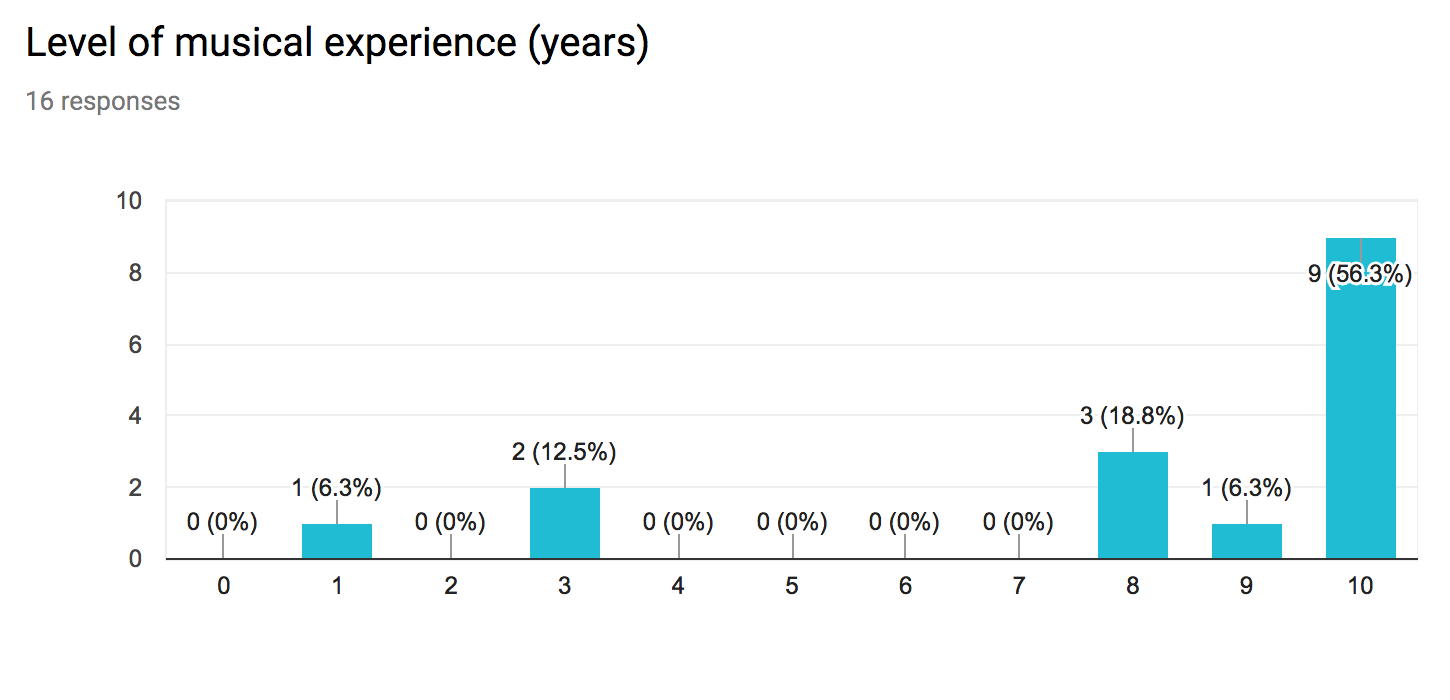
\includegraphics[width=\columnwidth]{musicExp}
    \caption{Musical Experience}
    \label{fig:musicExp}
\end{figure}
The instrumental breakdown can be seen in Figure \ref{fig:pieInst} below.
\begin{figure}[H]
    \centering
    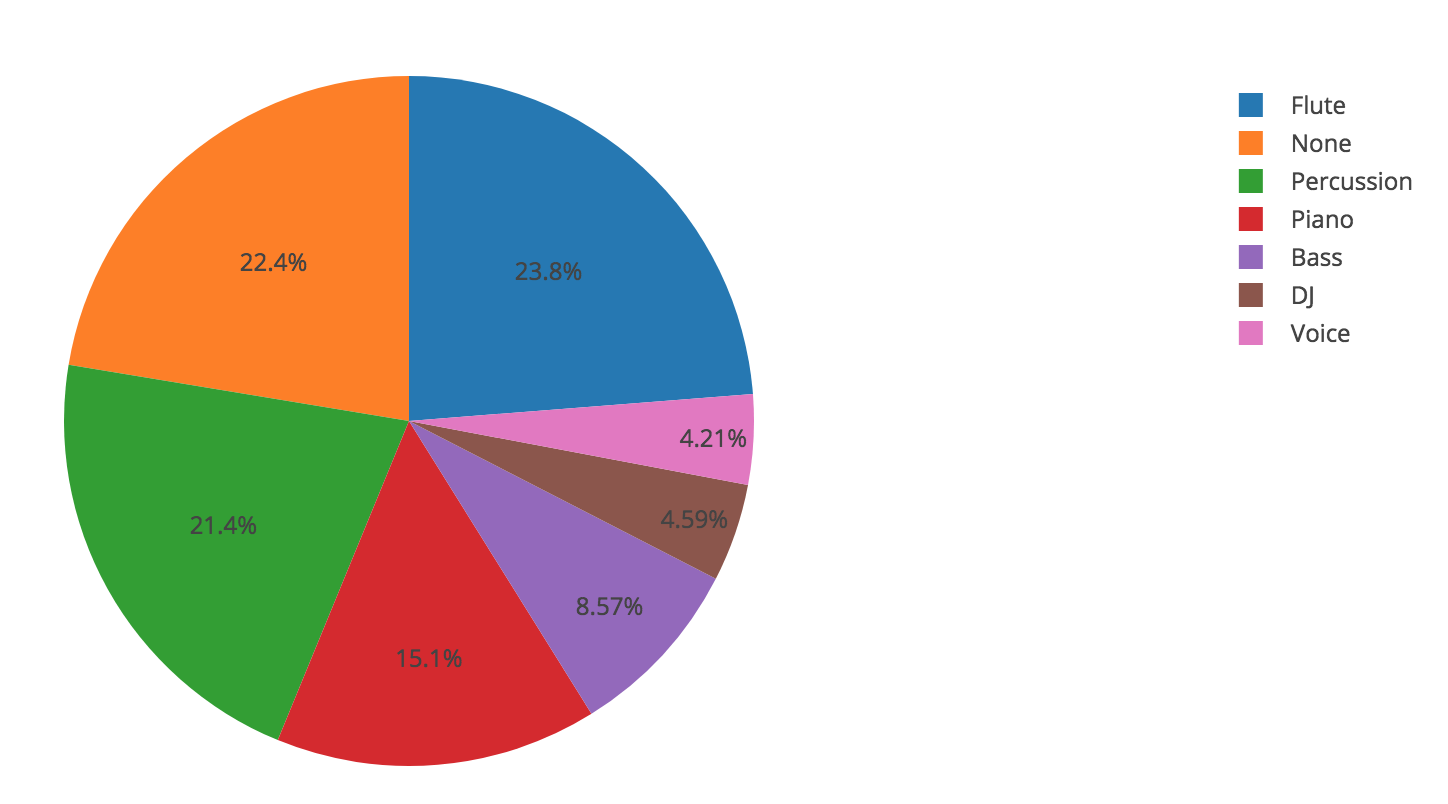
\includegraphics[width=\columnwidth]{pieInst}
    \caption{Spread of instrumental ability (out of 16)}
    \label{fig:pieInst}
\end{figure}
Thirteen users had some sort of prior experience with an audible metronome and three did not. For most this was their first experience with a haptic device. All users chose their dominant arm to wear the haptic sleeve and chose their dominant hand for tapping.
\begin{figure}[H]
    \centering
    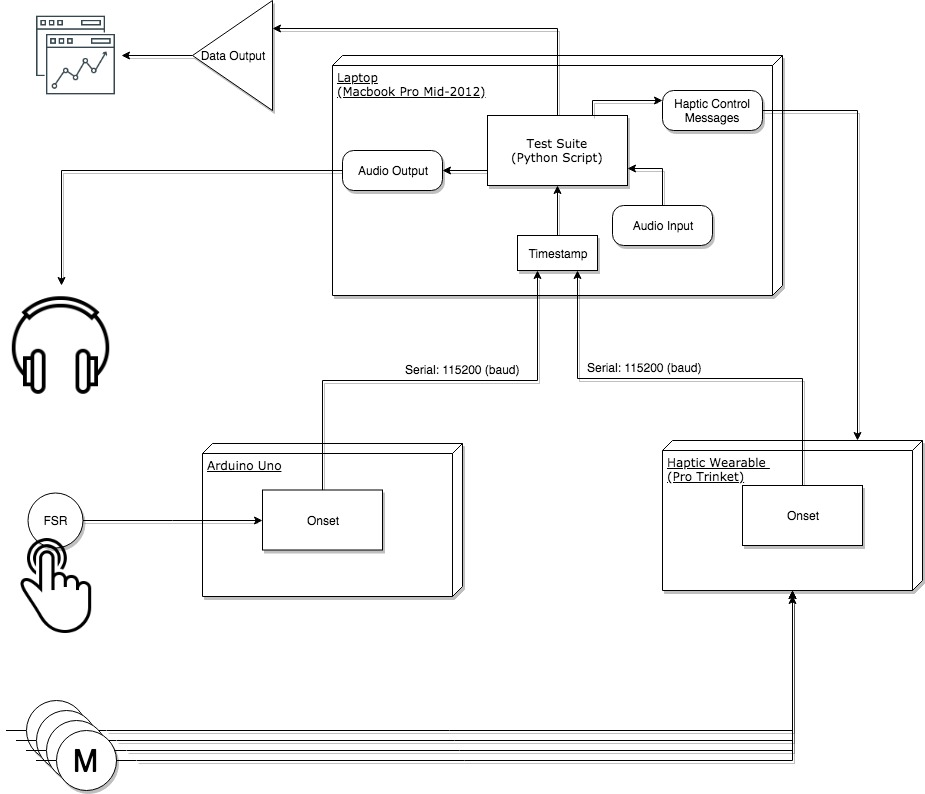
\includegraphics[width=\columnwidth]{TestSuiteFlowDiagram}
    \caption{Test Suite Flow Chart}
    \label{fig:TestSuiteFlowDiagram}
\end{figure}
\subsection{Setup} \label{testSetup}
To initialize setup, the subject is seated and given a pair of closed-back headphones. The FSR is situated to their preference and secured into place. Unlike a keyboard or button the FSR gives little to no feedback or rebound. This ensures a confident tap on each onset while providing no tactile response. The approach seeks to avoid intrinsic lag due to its independence of mechanical components. The delay limit is defined by the threshold applied in the software to avoid debounce, as discussed in Section \ref{development}

The Python file \textit{testSuite.py} is run and the UI will prompt the subject to input their name, read the instructions, agree to the conditions of the test suite, and commence with the test. The first 8 are practice tests to get used to the haptic sensation as well as the variety of audible test cases. The order of test case execution is scrambled with a static seed pseudo-random generator such that every user encounters the same test order. Every iteration of the test plots the Tap Onset, True Onset, and Sanitized Onset  for the purposes of feedback and affirmation of correct tapping as seen in Figure \ref{fig:TestCaseFeedbackEx}. Upon completion of the 48 test cases, the users are asked to fill out a survey for feedback.

\begin{figure}[H]
    \centering
    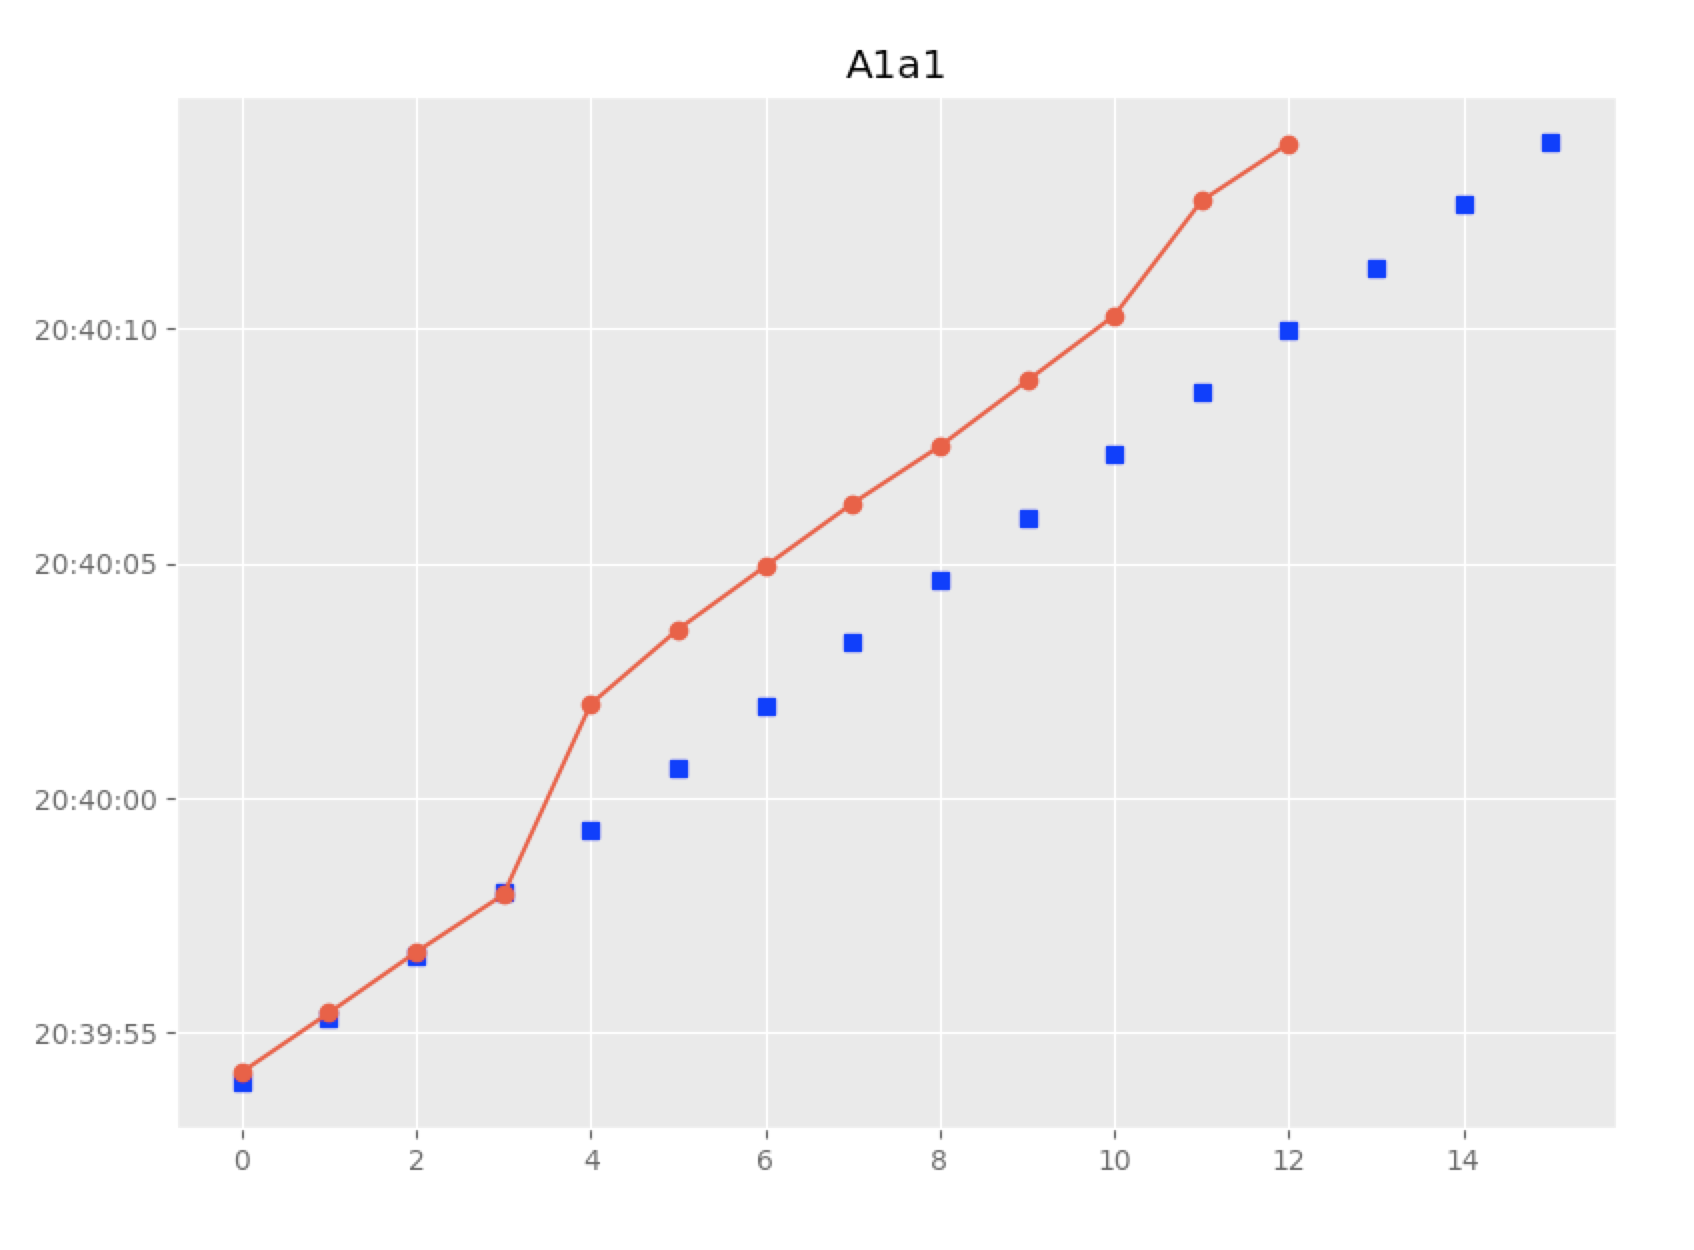
\includegraphics[width=\columnwidth]{TestCaseFeedbackExample}
    \caption{Test Case Feedback Example: Red circles are the tap onset, blue squares are the true onset. The x-axis is the tap count, the y-axis is elapsed time.}
    \label{fig:TestCaseFeedbackEx}
\end{figure}

\section{Results}\label{Results}
The main metric of stability and overall performance, as discussed in Section \ref{SMSTerms}, is the asynchrony. In all test cases a sanitization procedure was constructed to ensure that a missed tap would allow for the user to get back on track with the true onset later in the dataset - a process detailed entirely in Section \ref{sanitizationProcedure}. Finally, a latency correction factor was applied dependent on whether the test case was audible or haptic based. For more information on the derivation of this constant see Section \ref{latencyCalc}.

\subsection{SMS Research Expectations}
Prior SMS research has set expectations for the audible modality such that as the IOI increases the standard deviation of asynchrony $(SD_{asy})$ is expected to increase non linearly. This means that as we approach a slower bpm, we would anticipate larger deviations from the mean. This claim in in agreeance with the dataset across both modalities as shown in Figure \ref{fig:AllSummary} when viewing a subset of four test cases from right to left. For example, A3a1 relative to A3a2 through A3a4 and H1a1 compared to H1a2 through H1a4. These were test cases which had the highest inter-onset-interval and clearly exhibit high levels of variation relative to their adjacent test cases.
\begin{figure}[H]
    \centering
    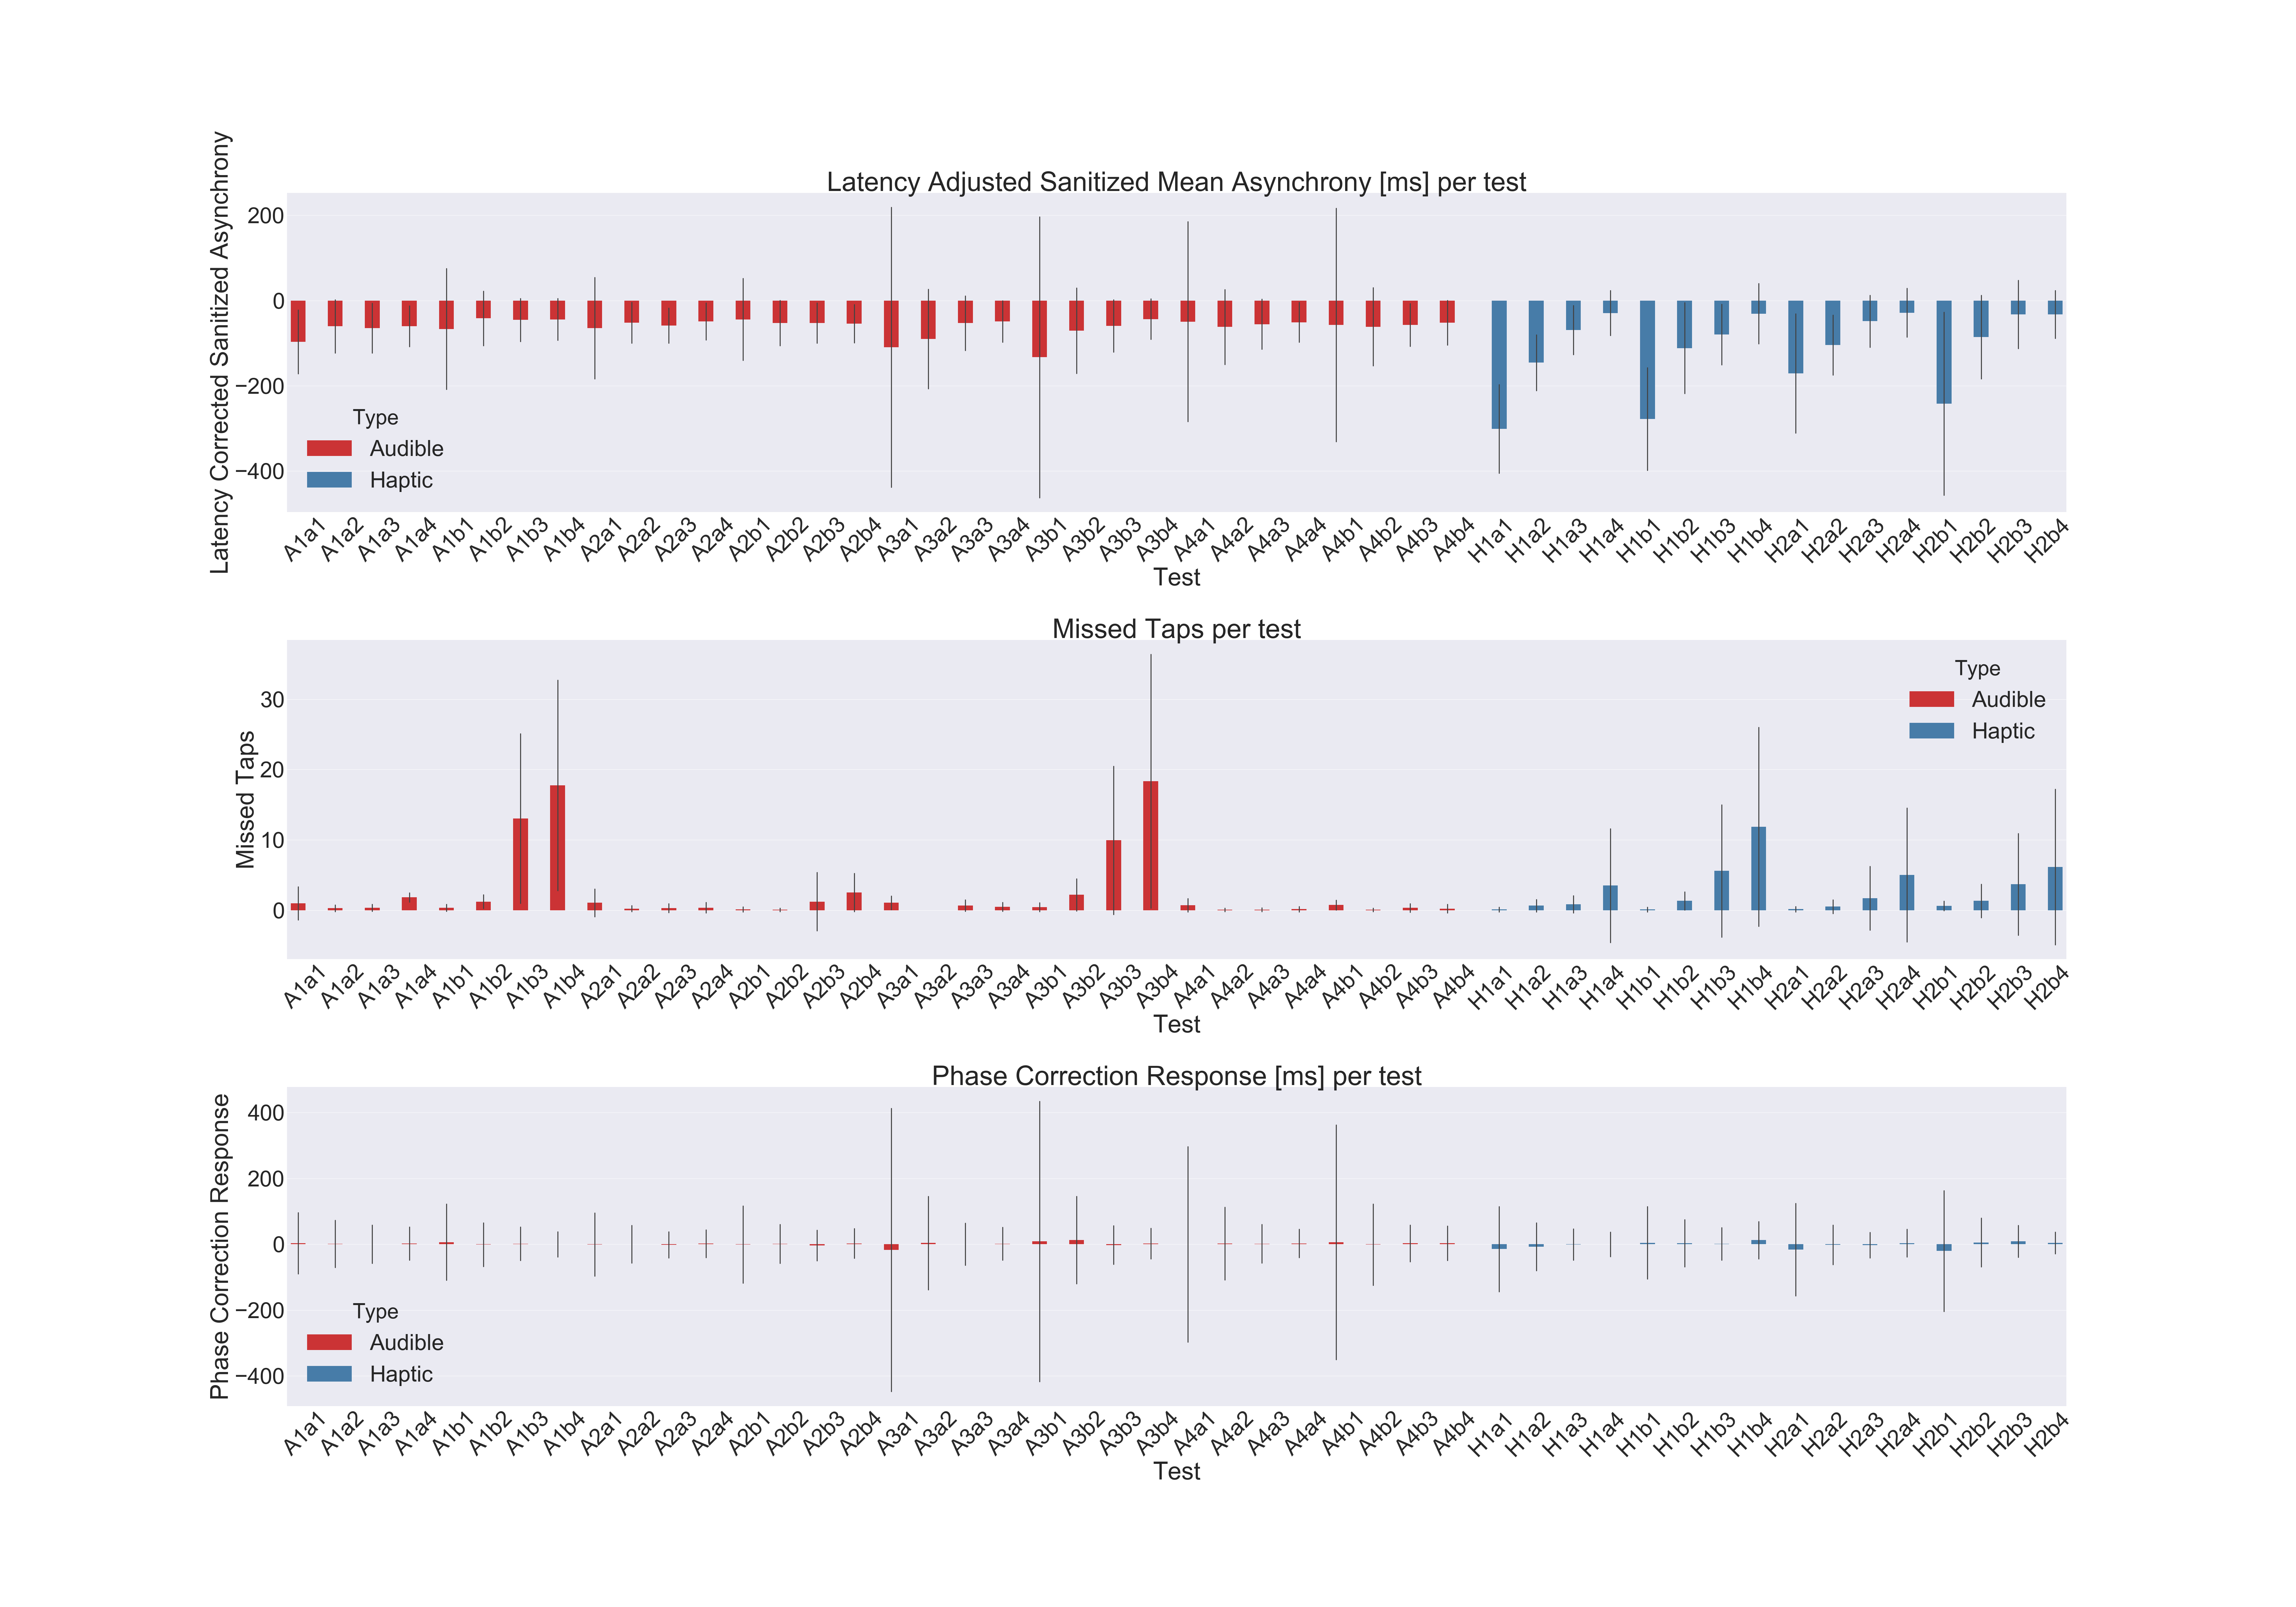
\includegraphics[width=\textwidth]{AllSummary}
    \caption{Summary across all participants}
    \label{fig:AllSummary}
\end{figure}

The black lines represent the standard deviation. The dynamic audible tests, A3a1 through A4b4, exhibited great deviation in both \textit{Latency Corrected Sanitized Asynchrony} (LCSA) and \textit{Phase Correction Response} (PCR), or the variation of one tap onset from the next.  The amount of metronomic jitter was varied on each repetition for these test cases and thus a reactionary response is expected since there was no real method of taking a proactive approach for these particular tests.

Most taps were missed during the interstitial legato chime or swing click A1b3, A1b4, A3b3, A3b4 as well as during the ramp up haptic test cases H1b3 and H1b4. These test cases ranged from 120 bpm to 180 implying either an indistinct onset, overstimulation, or low signal to noise ratio.

\subsubsection{Group Trends}
SMS findings anticipate a lower $(SD_{asy})$ for professionals compared to non musicians and expect little to no difference between amateurs and non musicians. As seen in Figure \ref{fig:GroupSummaries}, the results agree with prior research. Professionals had a mean LCSA of approximately -45 ms across all audible tests and approximately -75 ms for haptic tests relative to -55 and -90 ms for amateurs and -90 and -80 ms for non-musicians.

The non-professional group did marginally better on the haptic test cases than audible, though with a higher amount of missed taps. The standard deviation of the phase correction response, shown at the bottom of the figure, implies an ability to adapt tapping synchronization from beat to beat more successfully with the haptic device than across audible tests. This lends very promising insight but must be further classified to determine if the benefit is test case dependent or involving of strictly non-isochronous beats.
\begin{figure}[H]
    \centering
    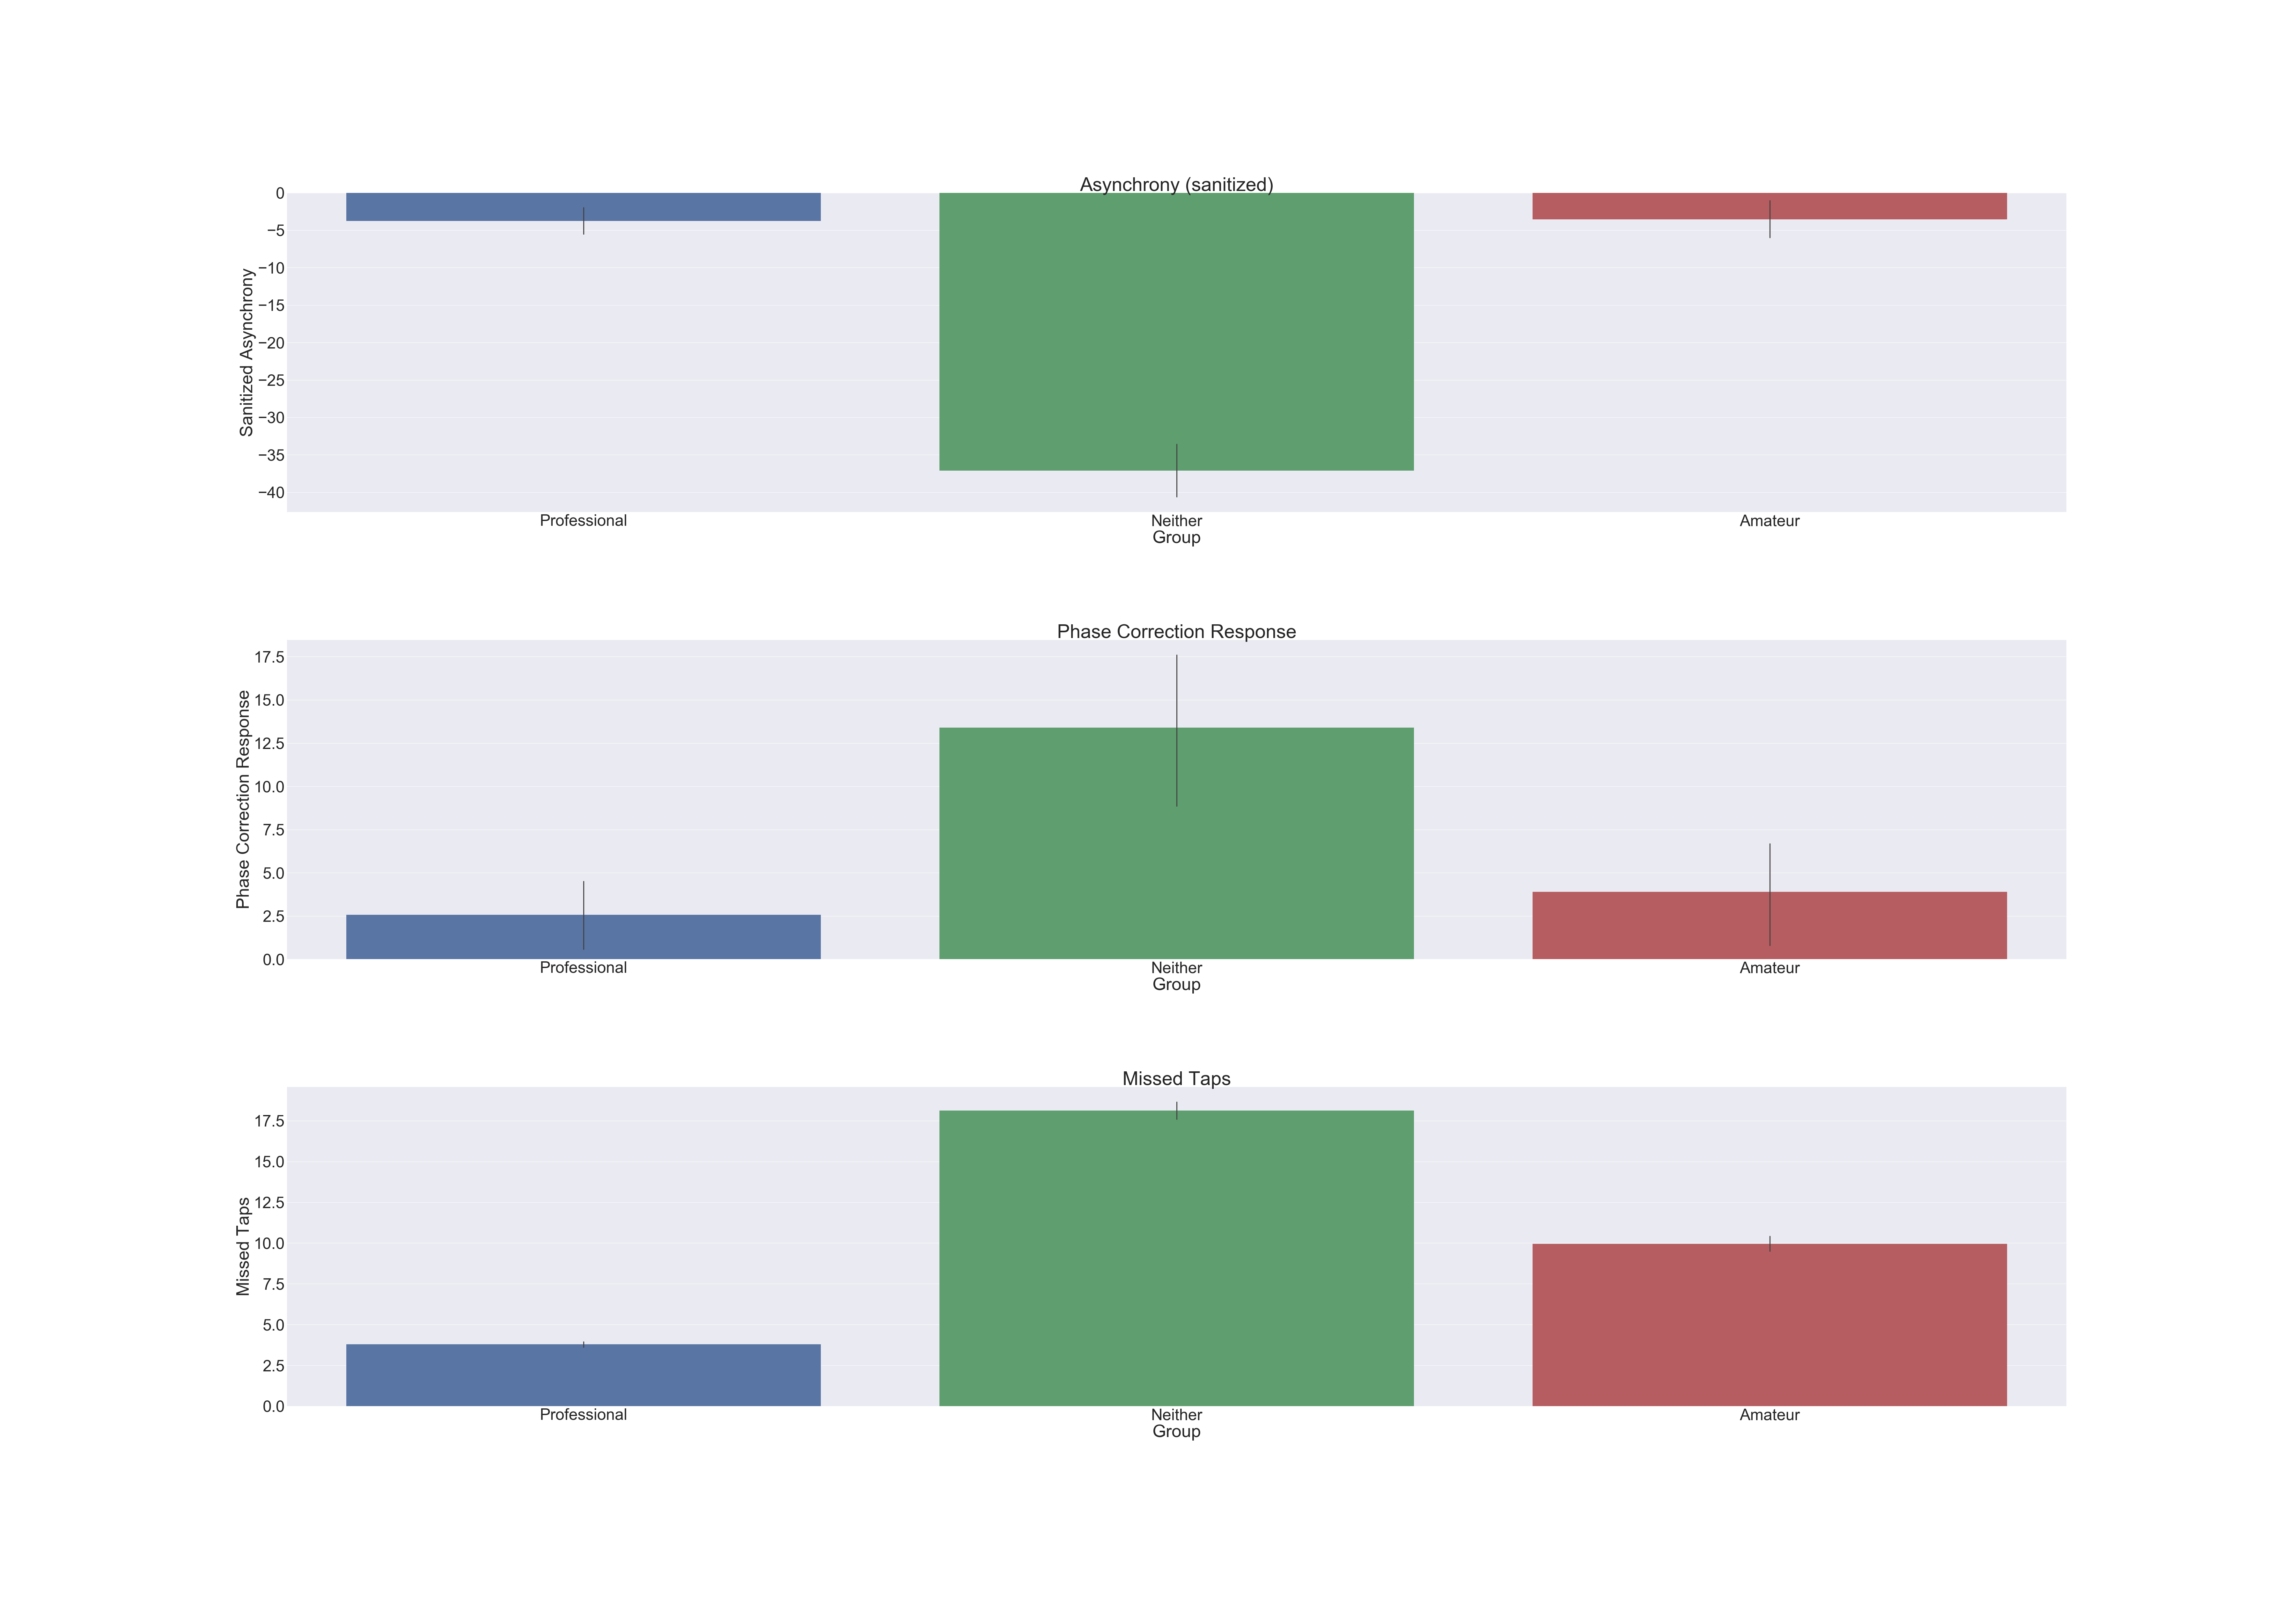
\includegraphics[width=\textwidth]{GroupSummaries}
    \caption{Group test summaries}
    \label{fig:GroupSummaries}
\end{figure}
\subsection{Instrumental Breakdown}

Past research into sensorimotor synchronization suggests a heightened rhythmic sensibility within percussionists and pianists who notoriously have held lowest variability values for tap tests. Figure \ref{fig:InstrumentSummaries} would suggest agreement with the exception of Bass. This is however, inconclusive, since the bins are uneven. For instance, whereas there was only a single bassist in the test, there were four percussionists. Without accounting for missed taps, it would appear that flutists held the lowest asynchrony across both modalities but the flutists were the group with the most missed taps for the haptic device. This could imply a negative interaction involving placement as these musicians are accustomed to a level of freedom on their arms.

\begin{figure}[H]
    \centering
    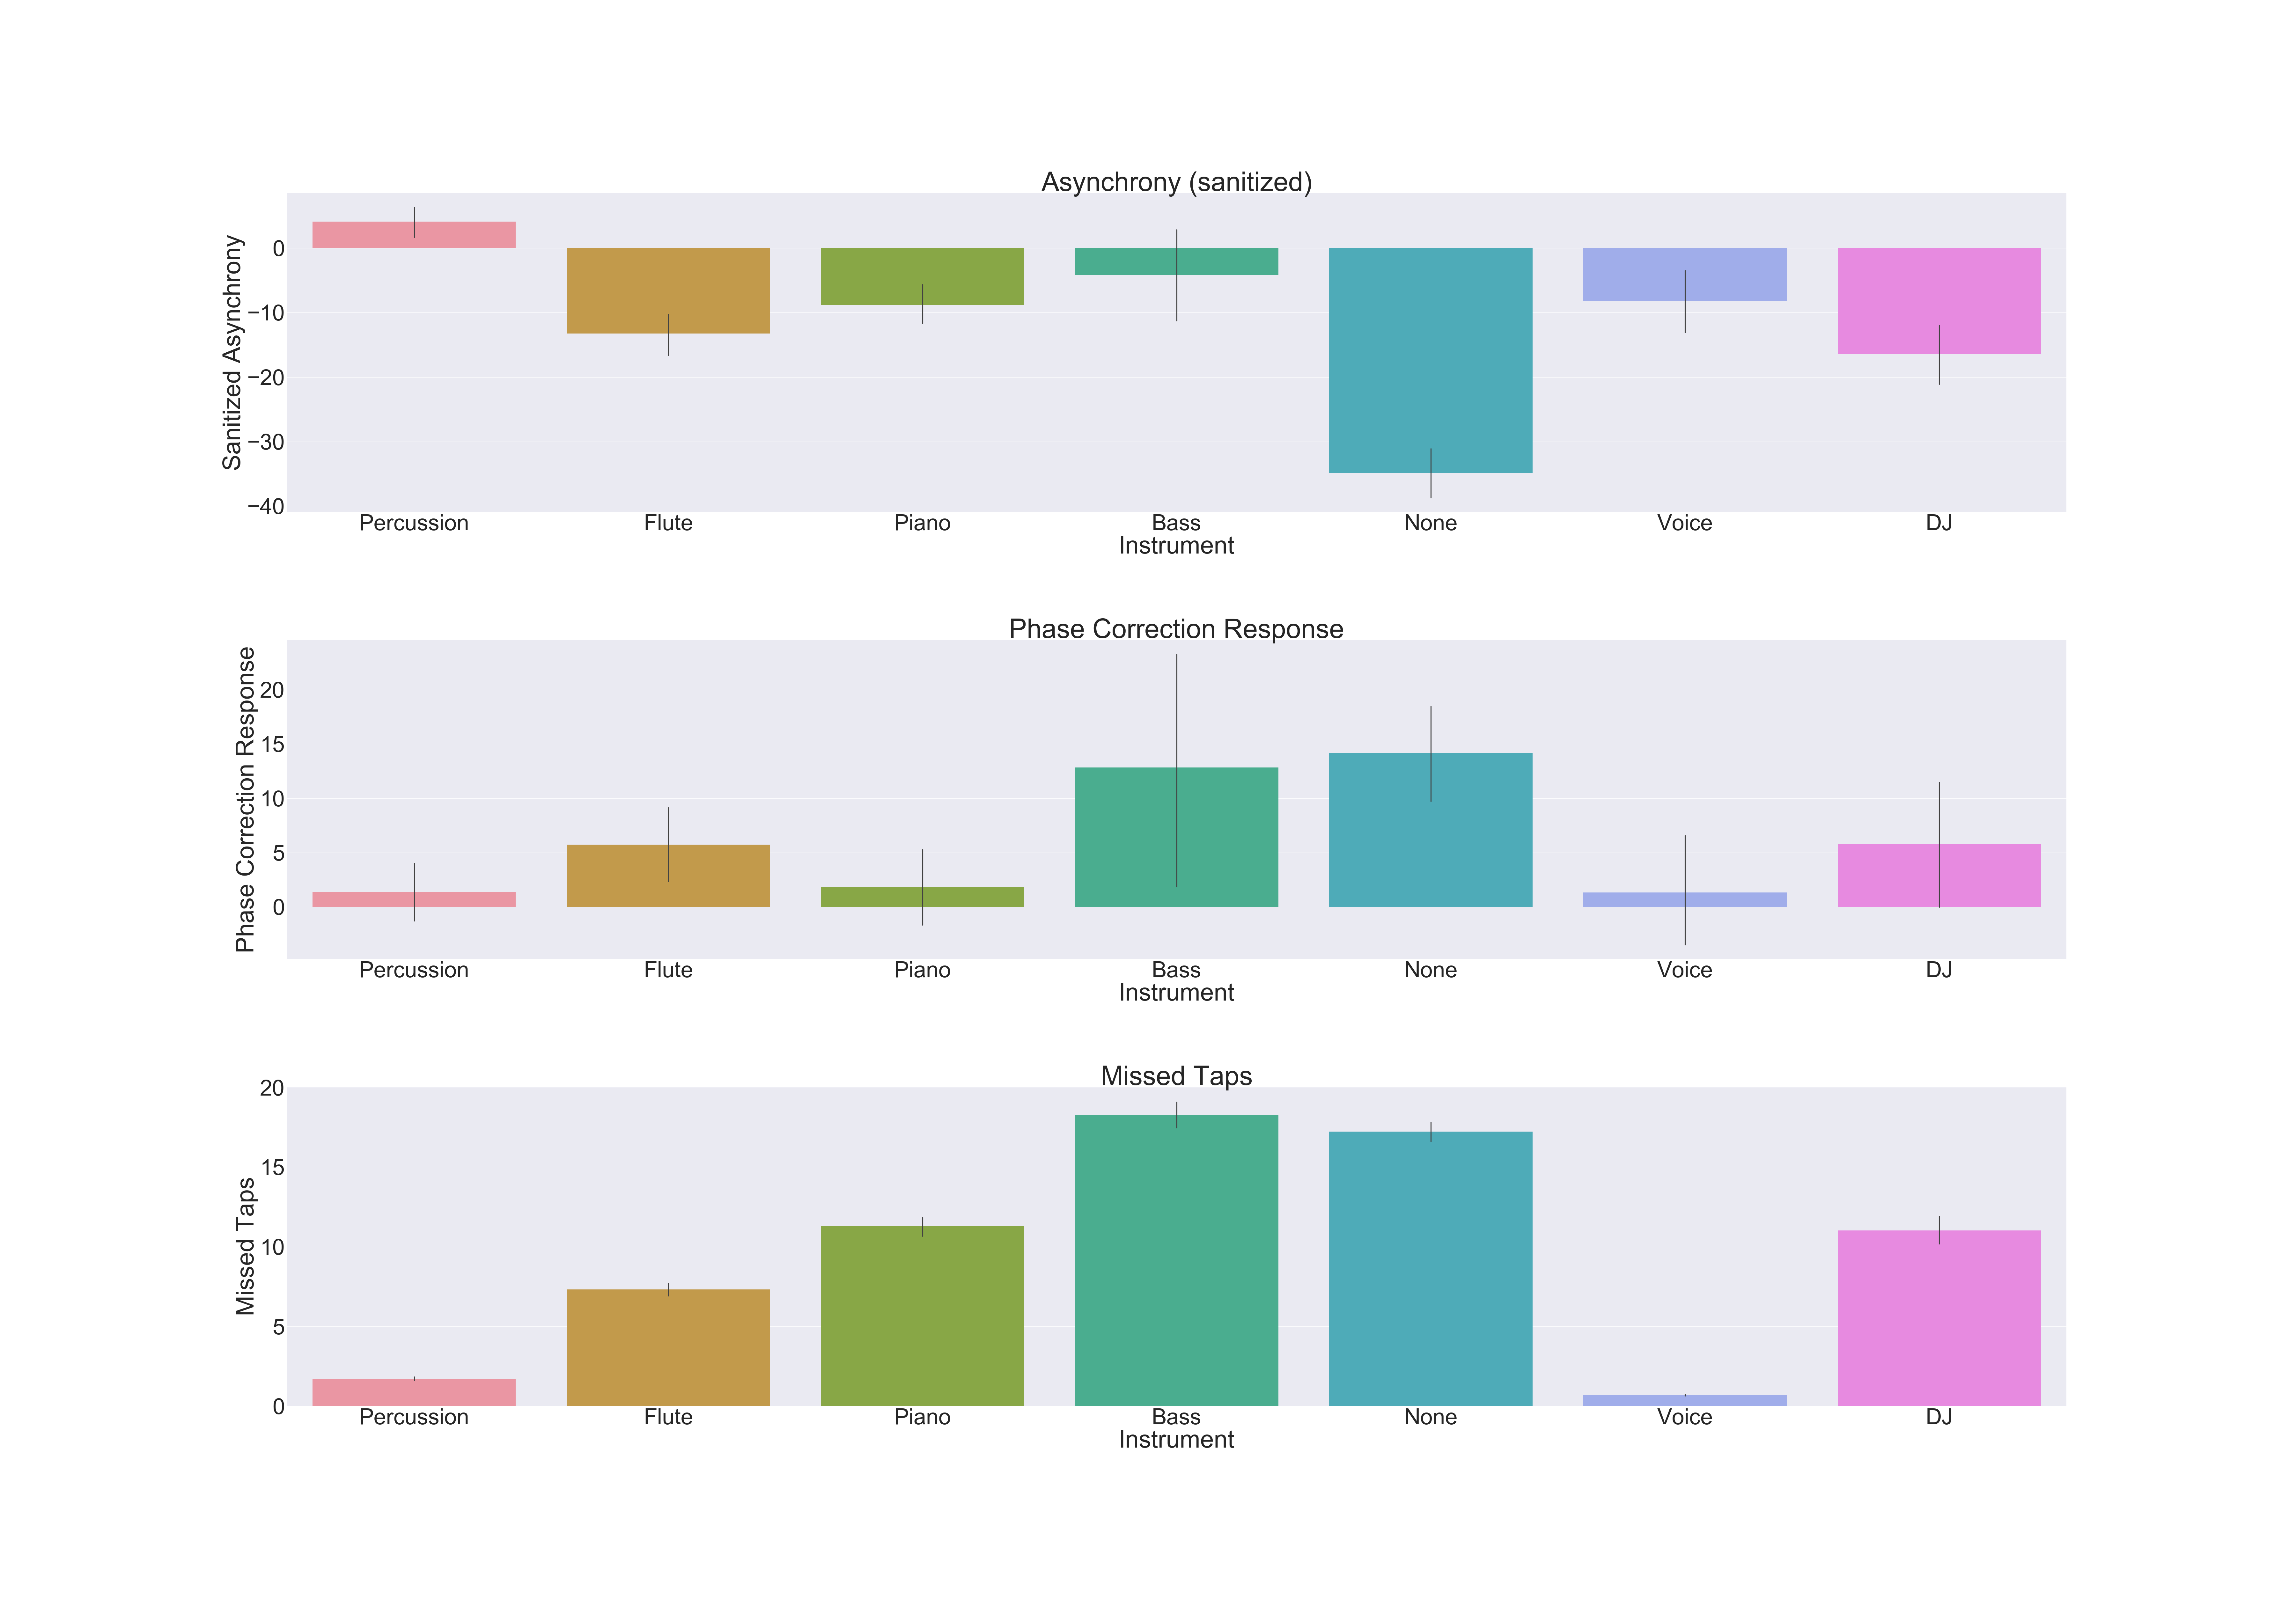
\includegraphics[width=\textwidth]{InstrumentSummaries}
    \caption{Summaries per instrument}
    \label{fig:InstrumentSummaries}
\end{figure}

\section{Haptic versus Audible Tests}
As expected, audible tests are the clear winner across all participants for the static test cases. As shown in \ref{fig:StaticComparison}, the mean of the audible tests is $-$56.92 ms with a standard deviation of 69.51 as compared to a mean of $-$92.67 ms with a much larger standard deviation of 109.29 for the haptic tests. With a delta of 35.75 ms between this would suggest that users are slightly more comfortable responding to isochronous beats with the auditory modality.
\begin{figure}[H]
    \centering
    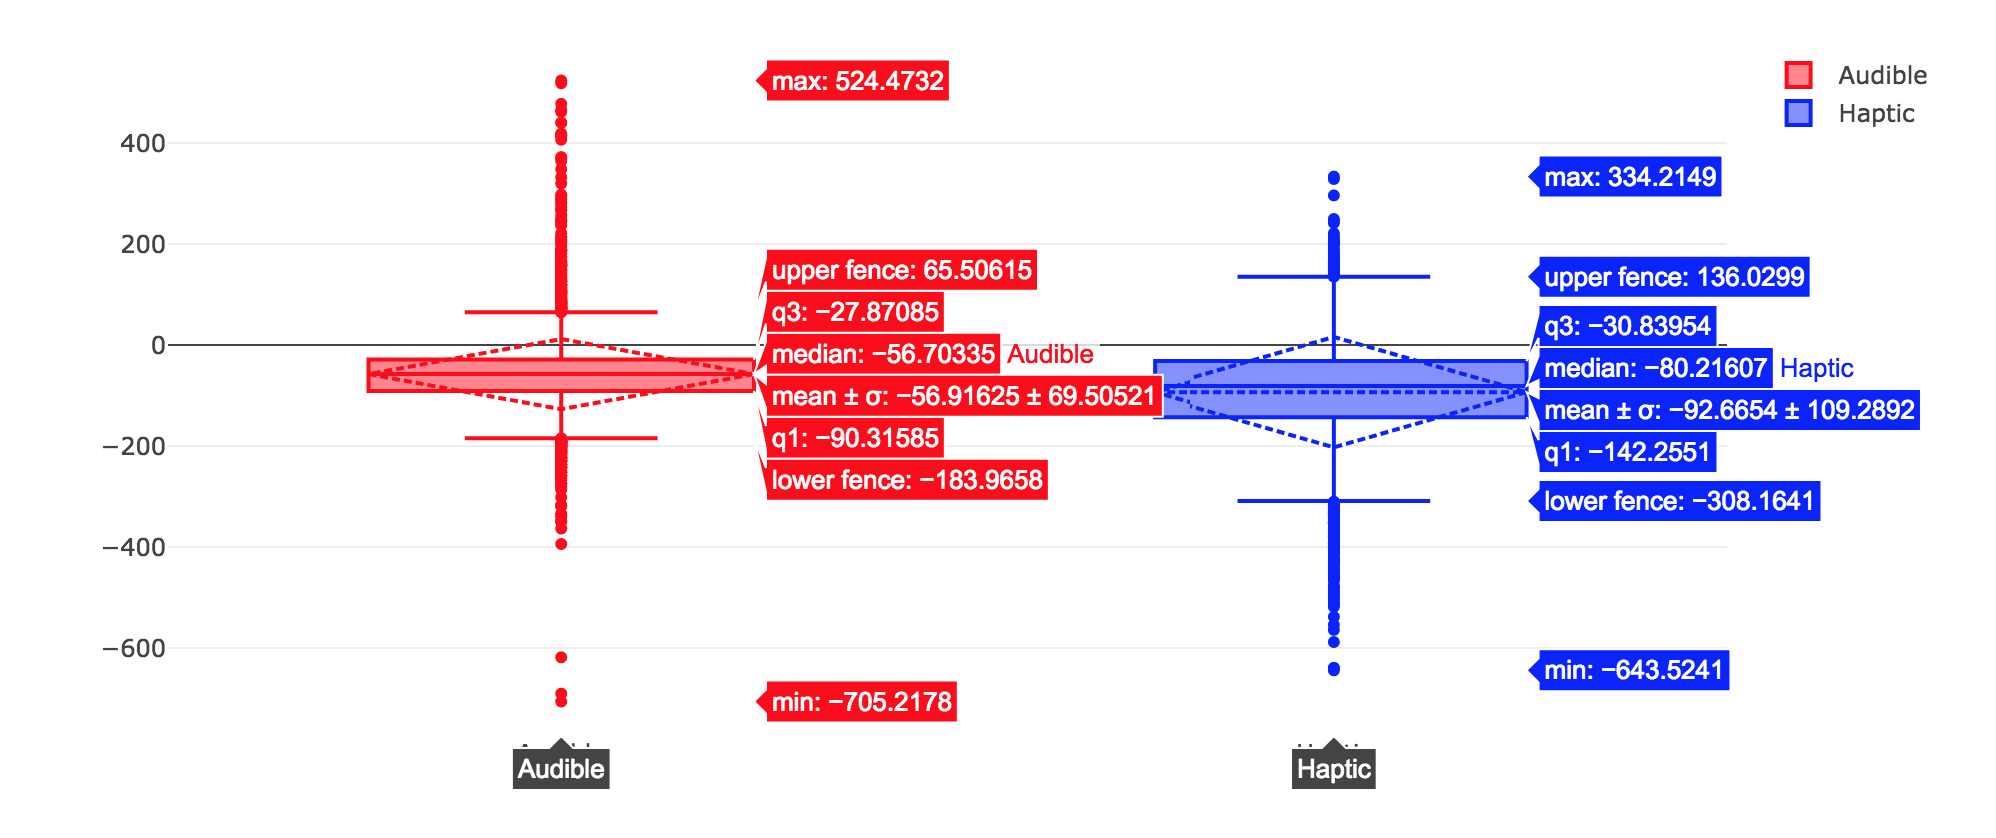
\includegraphics[width=\textwidth]{StaticComparison}
    \caption{Latency Corrected Sanitized Asynchrony for Static Tests}
    \label{fig:StaticComparison}
\end{figure}

The results are much more promising when comparing the dynamic test cases. As seen in Figure \ref{fig:DynamicComparison}, the haptic test results were a negligible 7.38 ms away from the audible but with a much cleaner standard deviation. This implies a greater synchronization ability with the haptic device and strongly supports the hypothesis of this work.

\begin{figure}[H]
    \centering
    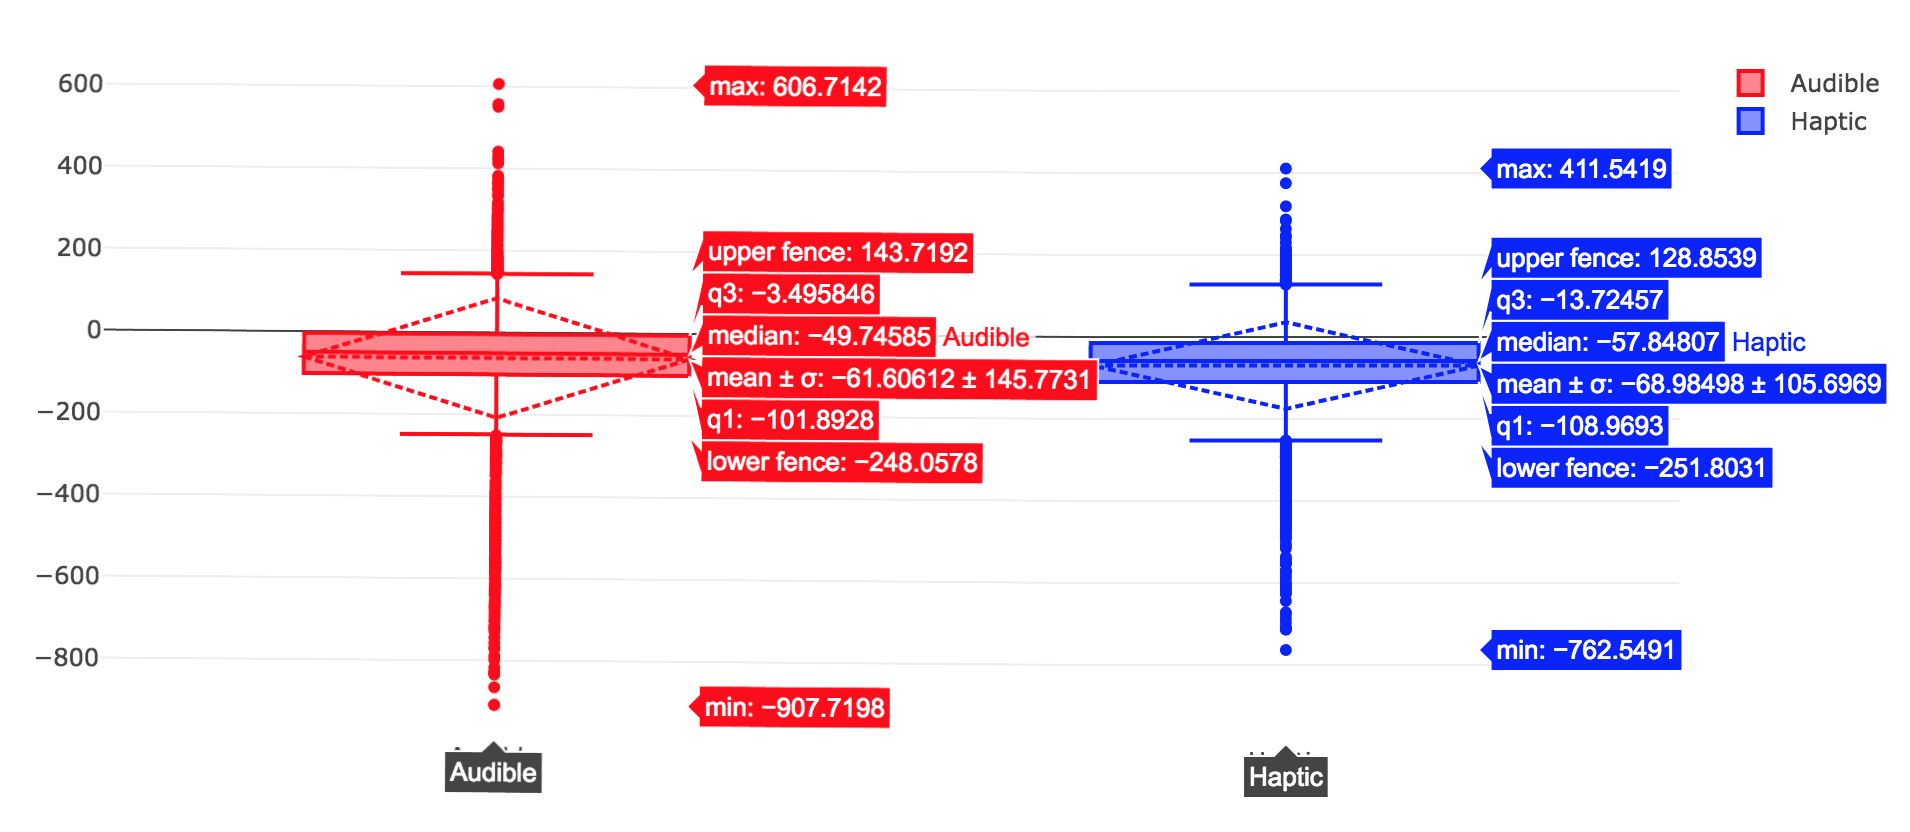
\includegraphics[width=\textwidth]{DynamicComparison}
    \caption{Latency Corrected Sanitized Asynchrony for Dynamic Tests}
    \label{fig:DynamicComparison}
\end{figure}

In a breakdown of asynchrony for static versus dynamic tests per group as shown in Figure \ref{fig:LCSA_KDE}, the dynamic haptic test cases exhibit a shift towards zero implying an improvement in synchronization during non-isochronous beats.   
\begin{figure}[H]
    \centering
    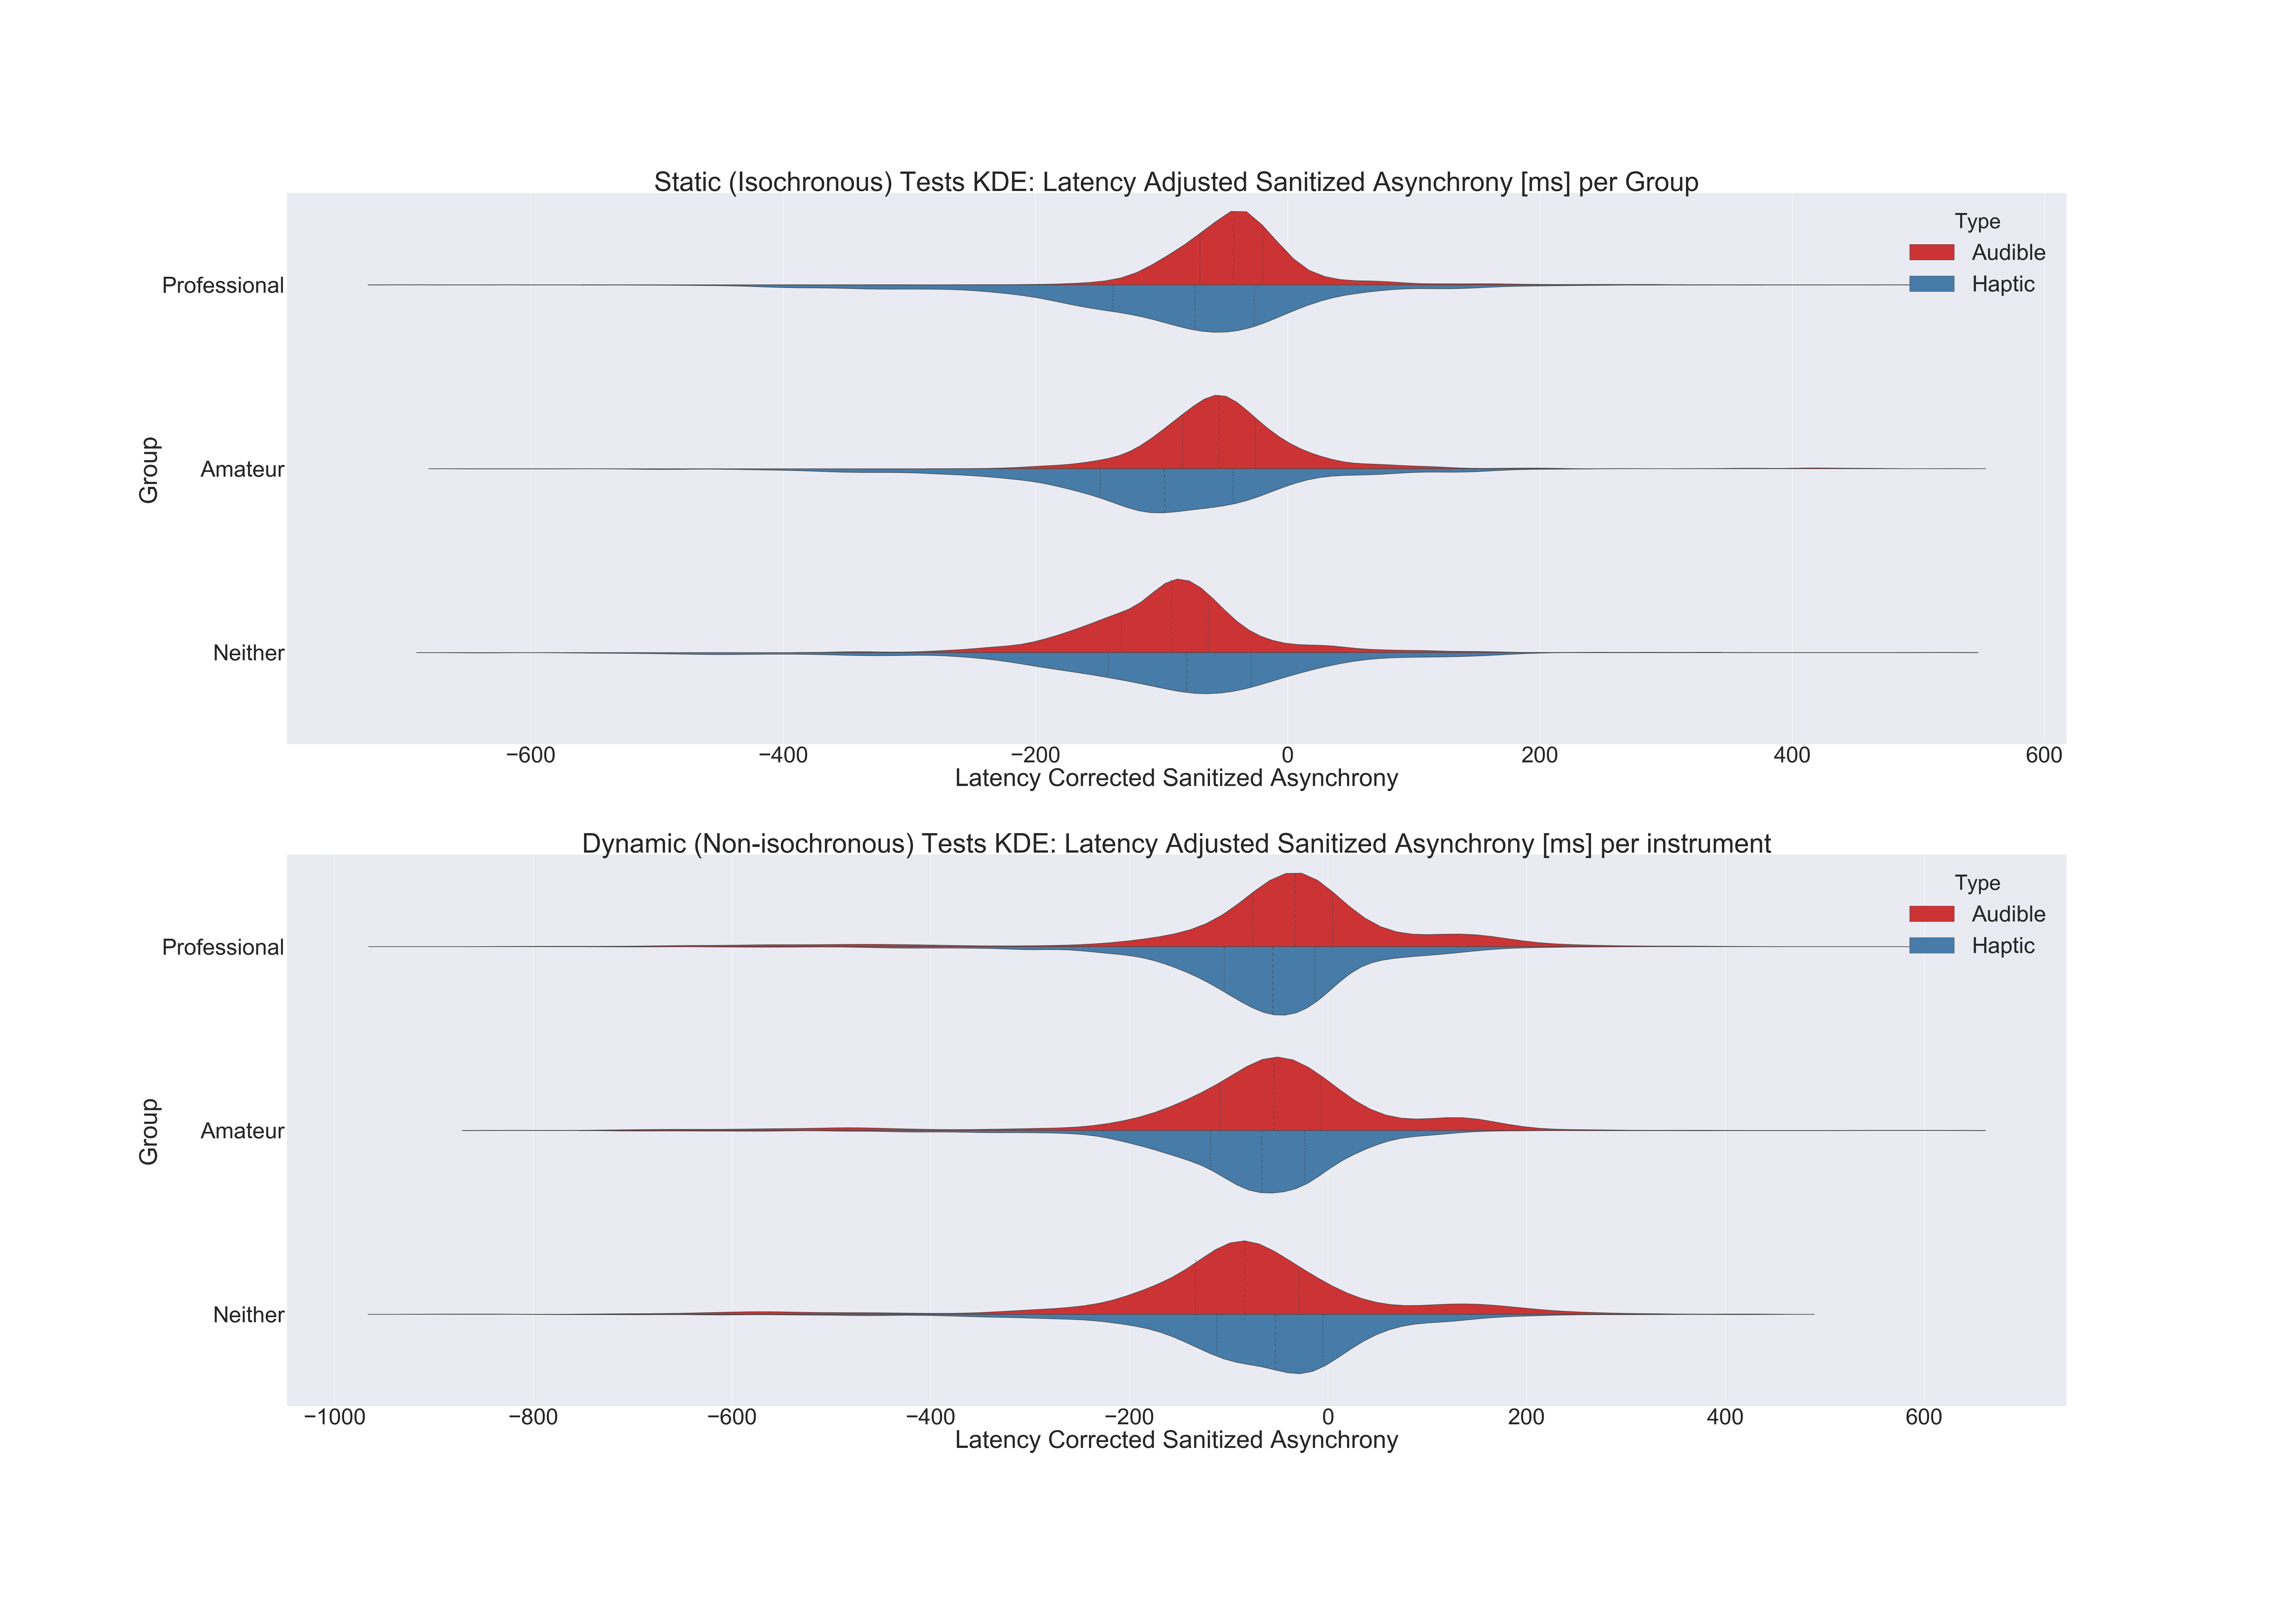
\includegraphics[width=\textwidth]{LCSA_KDE}
    \caption{Kernel Density Estimation: Latency Corrected Sanitized Asynchrony for Static vs Dynamic Tests}
    \label{fig:LCSA_KDE}
\end{figure}This finding heavily supports the overarching hypothesis of this work and can be further exemplified in Figure \ref{fig:sLCSAvIOI} and \ref{fig:dLCSAvIOI} below. As we traverse from left to right on the graph, the IOI increases - representing a decreasing bpm. The trajectory is nearly flat for the static audible test cases in red at the top. 
\begin{figure}[H]
    \centering
    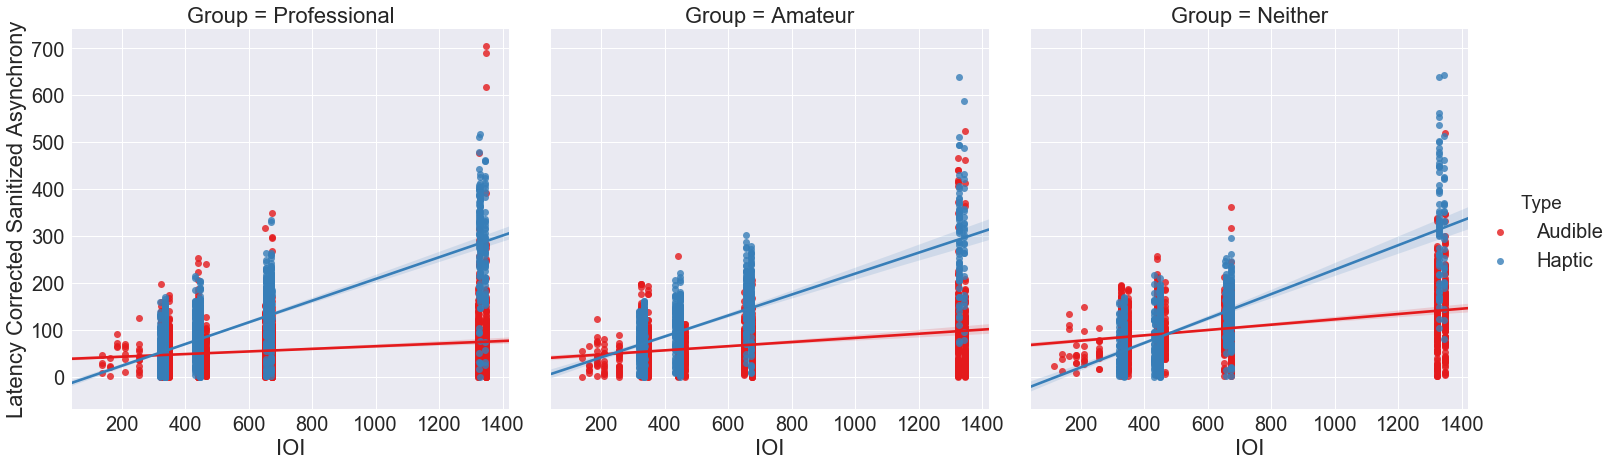
\includegraphics[width=\textwidth]{steady_LCSA_vs_IOI}
    \caption{Latency Corrected Sanitized Asynchrony vs. Inter-Onset-Interval across static test cases.}
    \label{fig:sLCSAvIOI}
\end{figure}
However, the dynamic audible tests trend towards a positive asynchrony implying a reactive approach. Near slower tempi the haptic tests contrarily trend steeply toward negative asynchronies in both the static and dynamic test cases. The deviation implies a proactive approach. The implications hint at an overall success for users to concretely navigate non-isochronous beats with the haptic metronome device. 
\begin{figure}[H]
    \centering
    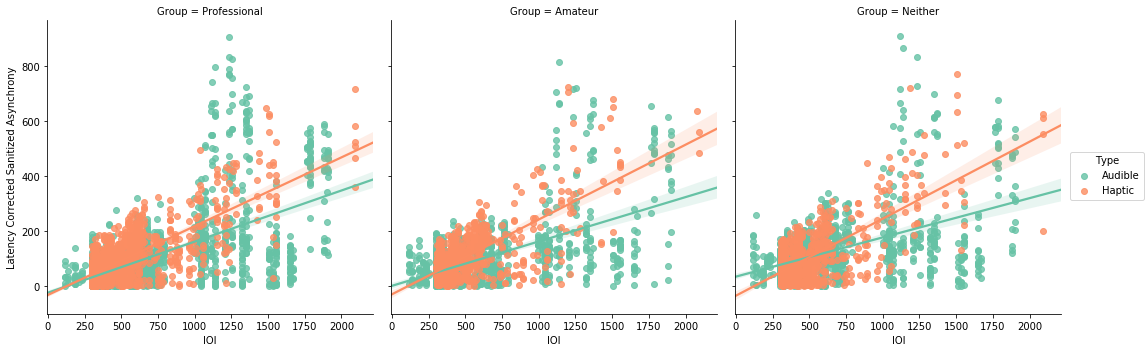
\includegraphics[width=\textwidth]{dynamic_LCSA_vs_IOI}
    \caption{Latency Corrected Sanitized Asynchrony vs. Inter-Onset-Interval across dynamic test cases.}
    \label{fig:dLCSAvIOI}
\end{figure}

\subsection{Haptic Poke versus Haptic Ramp}
To compare whether users were more inclined towards a particular mode of operation, either all on all off or ramp up ramp down, of the haptic and to check whether filling the interstitial space with the ramping sensation had any impact, the results in Figure \ref{fig:HPokevRamp} contrast the static and dynamic haptic instantaneous or poke test results to the haptic ramp method. The static haptic poke had an asynchrony of $-$93.17 $+/-$ 105.16. The static haptic ramp had an asynchrony of $-$92.12 $+/-$ 113.53. The delta is negligible and no conclusion can be made for a benefit within the isochronous realm for the haptic ramp. The dynamic haptic poke had an asynchrony of $-$69.93 $+/-$ 90.18. The dynamic haptic ramp had an asynchrony of $-$67.94 $+/-$ 120.43. A slightly better delta for the ramp sensation but a larger deviation implies that most users preferred the instantaneous sensation.
\begin{figure}[H]
    \centering
    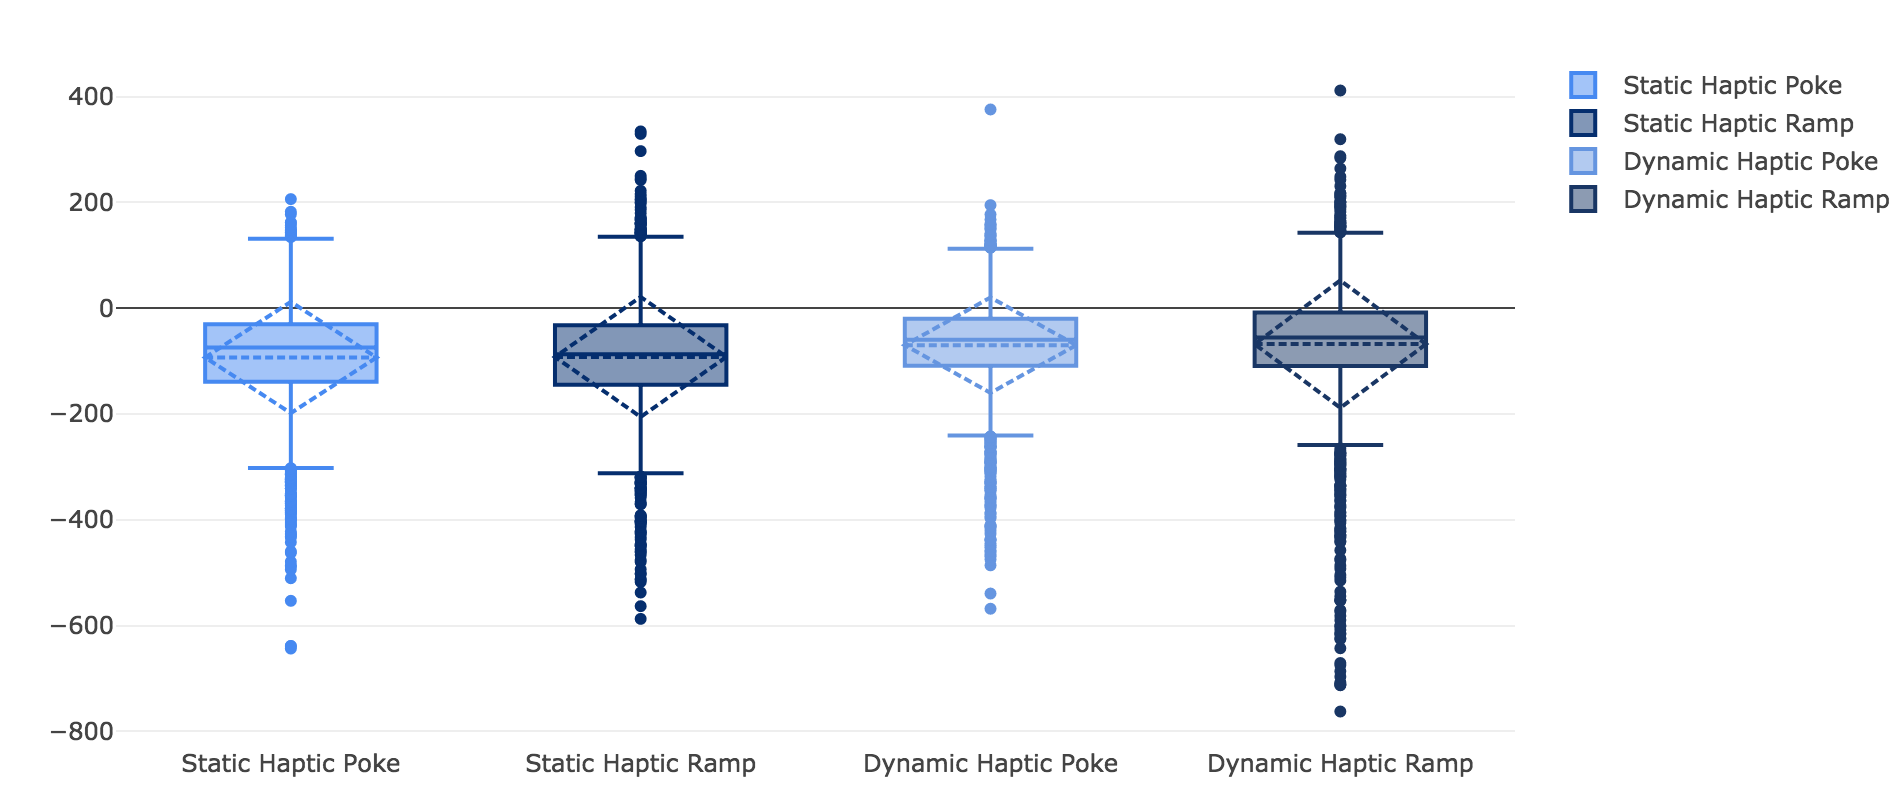
\includegraphics[width=\textwidth]{HPokevRamp}
    \caption{Latency Corrected Sanitized Asynchrony of haptic poke versus ramp effect across both static and dynamic tests.}
    \label{fig:HPokevRamp}
\end{figure}

\subsection{Audible Click versus Audible Music Tone}
To find out whether the legato audible music tone which saught to fill the interstitial space had any sort of favorable impact a mean comparison was conducted as shown in Figure \ref{fig:SDAudibleComparison}. The static audible click had a mean asynchrony of $-$59.47 with a deviation of 71.08 while the static audible musical tone was $-$53.46 $+/-$ 67.16. These results are so close that no improvement can be claimed.

The dynamic audible click had a mean asynchrony of $-$67.84 $+/-$ 152.39 while the dynamic audible musical tone had a mean asynchrony of $-$55.73 $+/-$ 138.98. From these results it would appear that there was a slight advantage when participants heard a musical tone that filled the interstitial space as opposed to a discrete click. 
\begin{figure}[H]
    \centering
    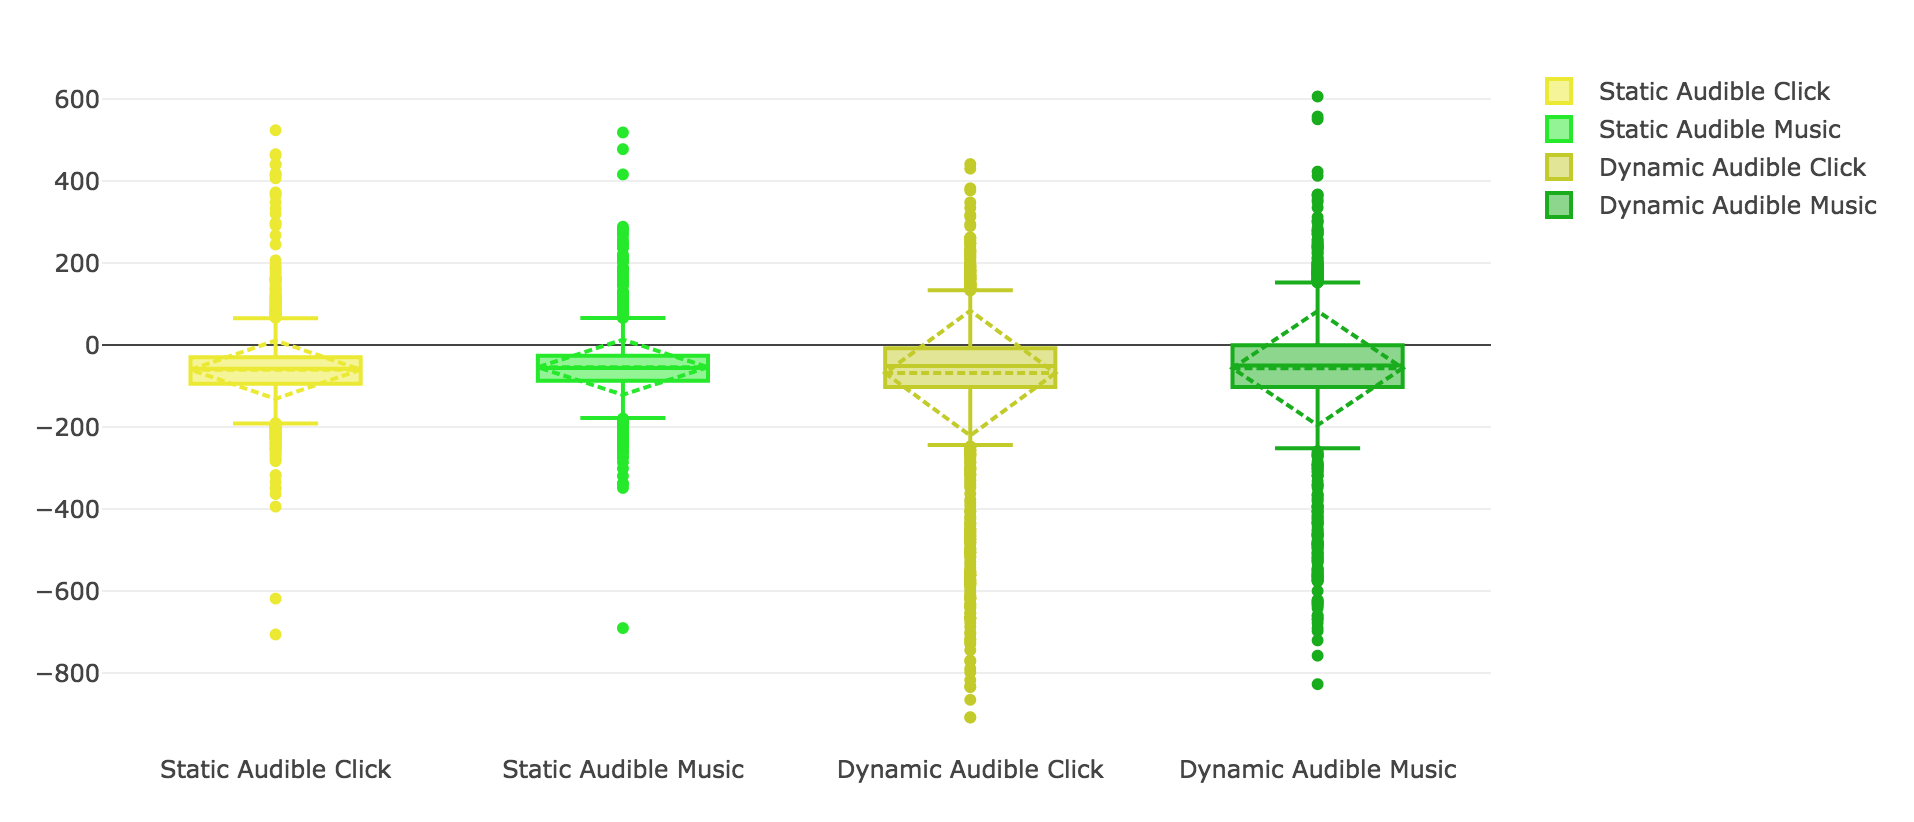
\includegraphics[width=\textwidth]{SDAudibleComparison}
    \caption{Latency Corrected Sanitized Asynchrony of audible click versus music tone across both static and dynamic tests.}
    \label{fig:SDAudibleComparison}
\end{figure}
\subsection{Analysis of variance across test cases}

To confirm the significance of the differences found between haptic and audible tests, an independent t-test with unequal variance was conducted. The null hypothesis was the assumption of no difference between these test case types in the latency corrected sanitized asynchrony value. P-values were obtained for haptic versus audible test case combinations across the static and dynamic groupings. The results are summarized in Figure \ref{fig:pvalue}.
\begin{figure}[H]
    \centering
    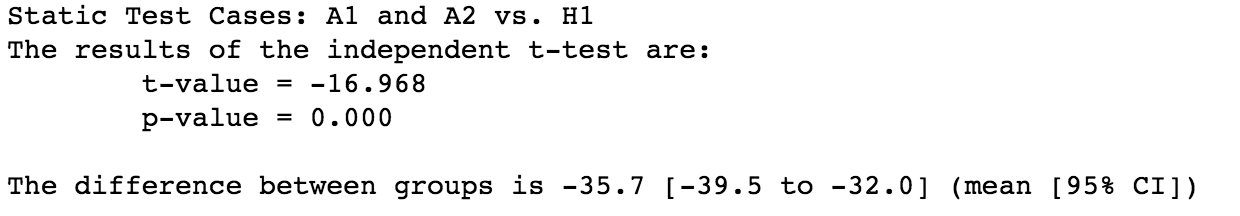
\includegraphics[width=\textwidth]{StaticP}
    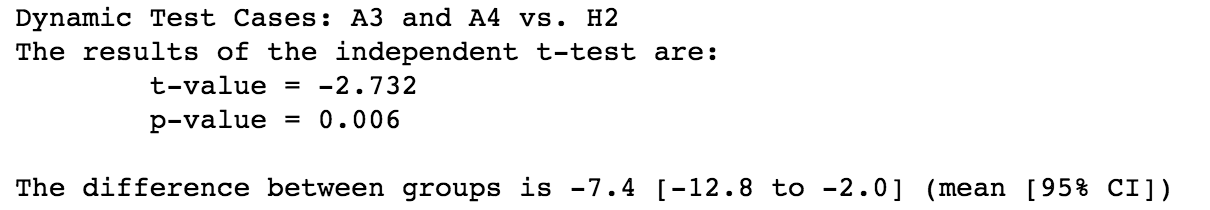
\includegraphics[width=\textwidth]{DynamicP}
    \caption{T-Test Results}
    \label{fig:pvalue}
\end{figure}
The extremely small p-value in both cases represents an overall success in negating the null hypothesis within a 95 percent confidence interval. This confirms that the variance of results between the static and dynamic tests cases for haptic and audible tests are indeed statistically significant and are not due to chance.

\section{Feedback}
On a scale of 1 to 10, with 10 being the most difficult, approximately 70\% of those tested found synchronization to the steady audible beat to be a level of 1, or extremely easy. The remaining 30\% found it to be either a 2 or 4 level of difficulty. However, the spread for dynamic audio test cases was much wider ranged, with the majority expressing a high level of difficulty 81.3\% above level 5 seen in Figure \ref{fig:Auddiff}. 
\begin{figure}[H]
    \centering
    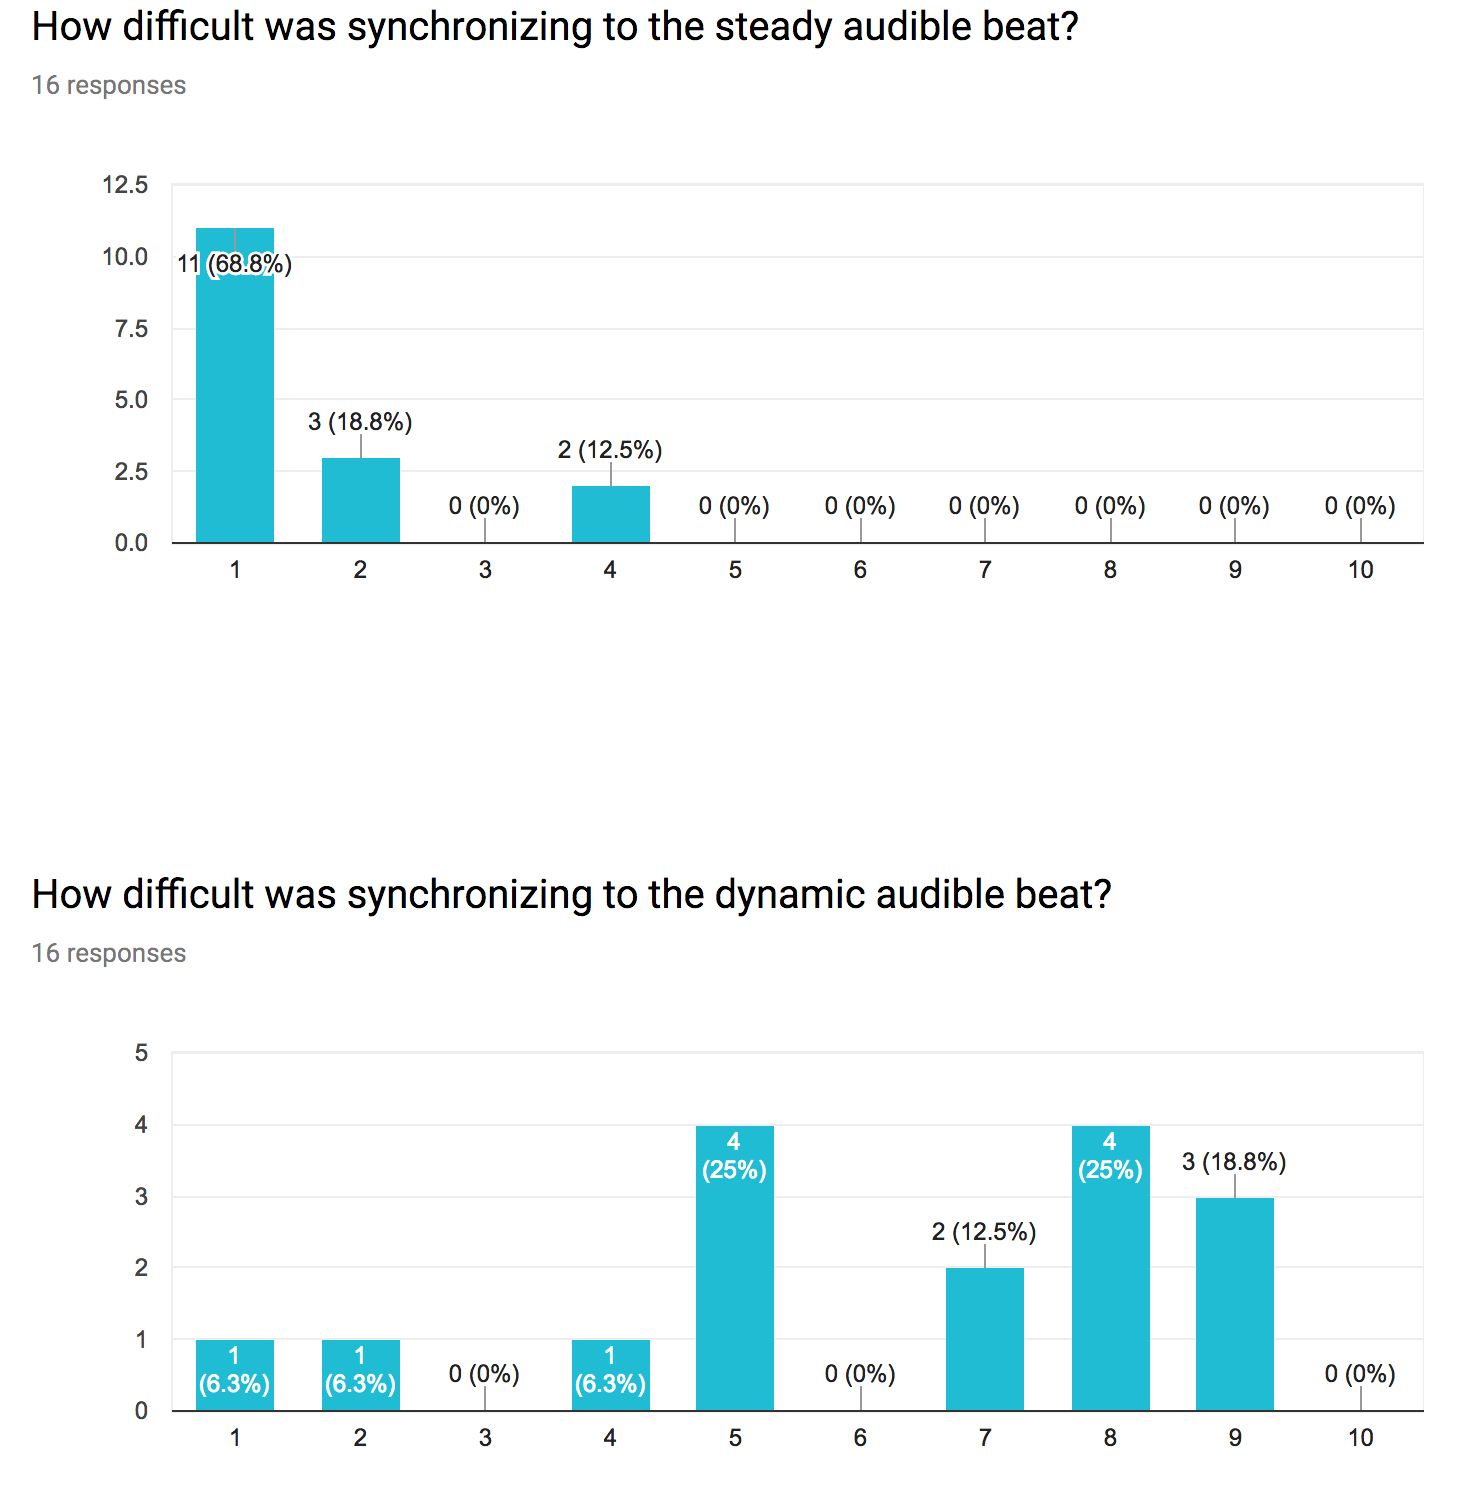
\includegraphics[width=\columnwidth]{Auddiff}
    \caption{Questionnaire: Difficulty results for dynamic audible tests.}
    \label{fig:Auddiff}
\end{figure}
The haptic tests had a wider difficulty spread across the steady beat shown at the top of Figure \ref{fig:Hapdiff}. This was to be expected as users had no prior experience with this haptic device let alone any other sort of wearable metronome. If retested or trained over the course of a few weeks to the sensation of touch the responses might have been more favorable or closer in resemblance to the static audible tests. Future experiments could involve a retest of participants after an acclimation period to determine whether adaptation to the haptic sensation prevailed. Regardless, the dynamic beat for the haptic modality yielded less difficulty rankings than the dynamic audible (11 ranked a level of 5 or more difficulty vs. 13 for audible dynamic tests), which further supports the hypothesis of this work.
\begin{figure}[H]
    \centering
    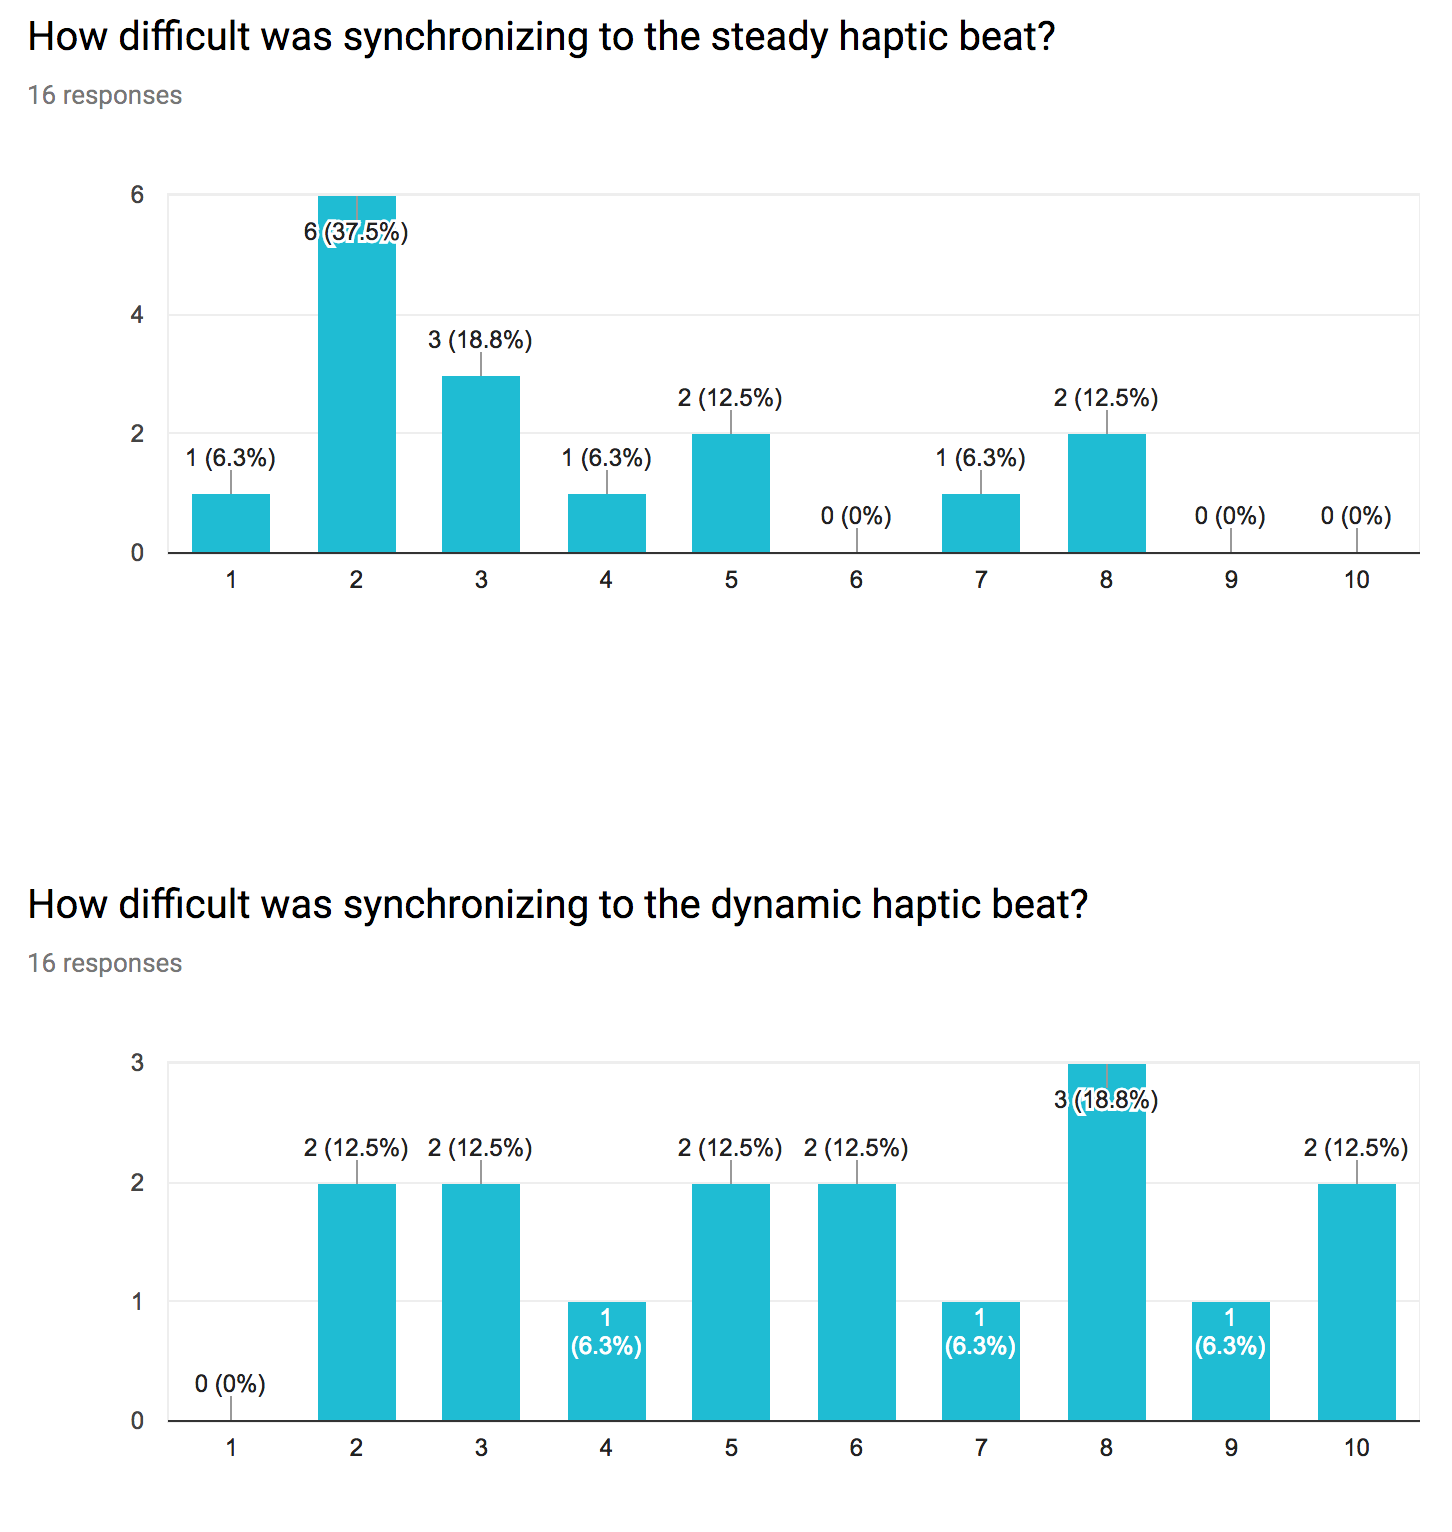
\includegraphics[width=\columnwidth]{Hapdiff}
    \caption{Questionnaire: Difficulty results for dynamic haptic tests.}
    \label{fig:Hapdiff}
\end{figure}

With the question of modality preference, auditory won hands down for the steady beat. Some users would have preferred a combination of both auditory and haptic, though the option was not exemplified in the test suite. The haptic won by 13\% for the dynamic tests, shown in Figure \ref{fig:modPref}
\begin{figure}[H]
    \centering
    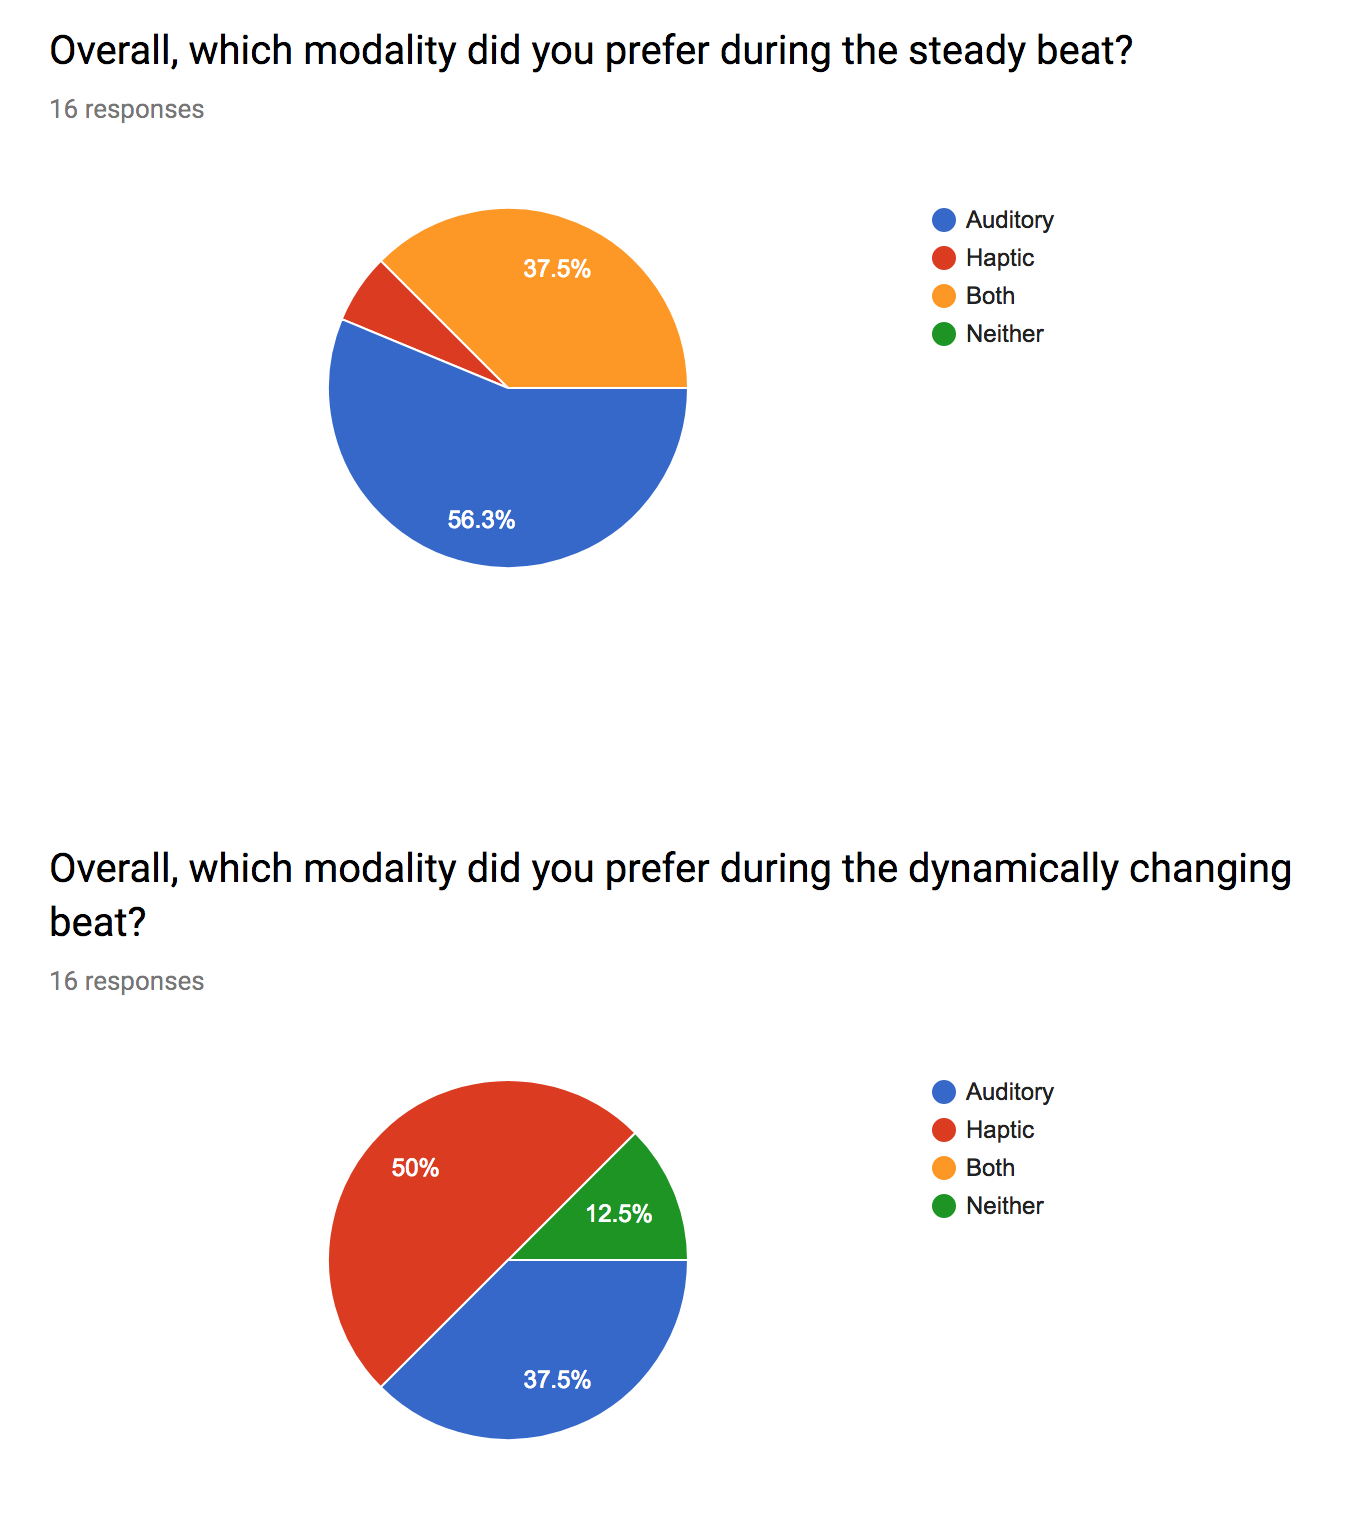
\includegraphics[width=\columnwidth]{modPref}
    \caption{Questionnaire: Modality preference}
    \label{fig:modPref}
\end{figure}

When asked specifically about the preference for haptic mode of operation, it seemed that most users preferred the all on all off mode see in Figure \ref{fig:hspace}
\begin{figure}[H]
    \centering
    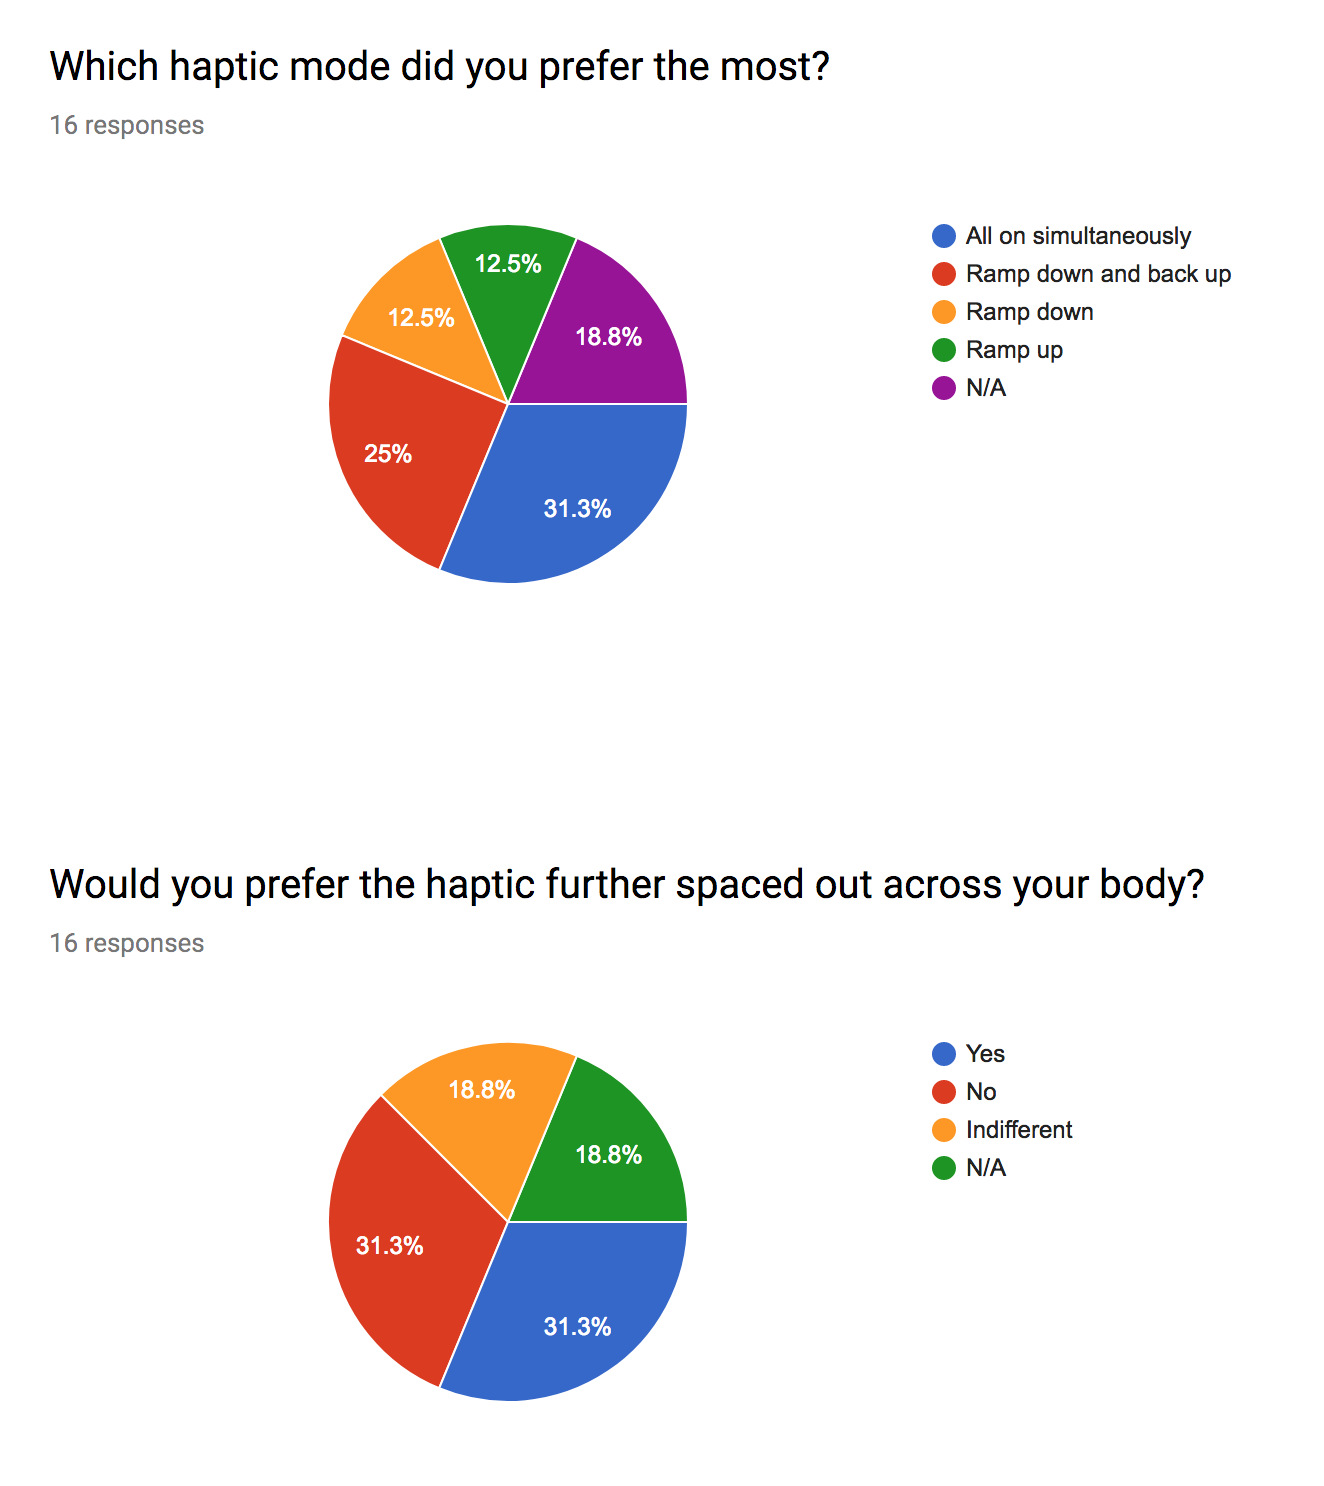
\includegraphics[width=\columnwidth]{hspace}
    \caption{Questionnaire: Haptic mode preference and spacing}
    \label{fig:hspace}
\end{figure}

This could be attributed to the lack of stimulation strength at higher vibrating frequencies for the ramping mode, an intrinsic flaw due to the nature of power operation of the haptic prototype at 5 V 500 mA laptop USB max output. This would be remedied in the next design iteration discussed in \ref{wirelessHP}. 

Furthermore, the users were tested at up to (and occasionally past) 180. This is well beyond the documented 150 bpm limit. At such rapid speeds the vibrotactiles had little time to ramp up to full capacity. This was another reason for diminished strength and could have possibly yielded a sensation nearly indistinguishable from noise.

When asked about placement preference, there was a 31.3\% split between the desire to have it further spaced or not. Prior research advocates a larger area of coverage to isolate stimulation zones and promote perceptivity. This would be adopted in a more flexible way in the next prototype iteration with velcro straps spaced out to the desired length.

\section{Conclusions}
Overall, the results are quantitatively promising in support of the hypothesis that filling in the interstitial space provides benefit for non-isochronous or dynamic beats.